\documentclass[a4paper]{article}
\usepackage{hyperref}
\hypersetup{
    colorlinks=true,
    linkcolor=black
}
\usepackage{amsmath}
\newcommand{\qed}{\hfill $\Box$}
\usepackage{mathrsfs}
\usepackage{bm}
\usepackage{tikz}
\usetikzlibrary{patterns}
\usetikzlibrary{positioning}
\usetikzlibrary{arrows.meta}
\setlength{\parindent}{0pt}
\usepackage[most]{tcolorbox}
\tcbset{
    enhanced,
    colback=white,
    colframe=black!80,
    fonttitle=\bfseries\color{white},
    drop shadow=gray
}
\usepackage{geometry} 
\geometry{left=2cm,top=2cm,right=2cm,bottom=2cm}
\usepackage{amsfonts}
\usepackage{amssymb}
\usepackage{multicol}
\usepackage{setspace}
\usepackage{enumerate}
\usepackage{colortbl}
\usepackage{relsize}
\usepackage{exscale}
\usepackage{xcolor}
\usepackage{listings}
\usepackage{tabularx}
\usepackage{pgfplots}

\definecolor{codegray}{gray}{0.9}
\definecolor{codeblue}{RGB}{41,5,195}
\definecolor{codegreen}{RGB}{30,150,30}
\definecolor{codepurple}{RGB}{127,0,85}
\definecolor{backcolour}{rgb}{0.95,0.95,0.92}

\lstdefinestyle{mystyle}{
backgroundcolor=\color{backcolour},
commentstyle=\color{codegreen},
keywordstyle=\color{codeblue},
numberstyle=\tiny\color{codegray},
stringstyle=\color{codepurple},
basicstyle=\ttfamily\footnotesize,
breakatwhitespace=false,
breaklines=true,
captionpos=b,
keepspaces=true,
numbers=left,
numbersep=5pt,
showspaces=false,
showstringspaces=false,
showtabs=false,
tabsize=2
}

\lstset{style=mystyle,language=Python}


\title{\textbf{Algorithm1}}

\begin{document}
\maketitle
\thispagestyle{empty}
\pagebreak



\tableofcontents
\pagenumbering{roman}
\pagebreak

\pagenumbering{arabic}
\section{Fundamentals}
\subsection{Steps to Developing Algorithms}
\begin{enumerate}
    \item Modelling the problem
    \item Define data structures and algorithms to solve it
    \item Define and analyse cost
    \item Iterate until satisfied
\end{enumerate}

\subsection{Analysis of Algorithms}
\subsubsection*{Observation} (But usually you can't afford to build the full solutions and run it multiple times)
\begin{spacing}{1.5}
\begin{tabularx}{0.9\textwidth}{X|X}
    \hline
    \textbf{System independent factors} & \textbf{System dependent factors} \\
    \cline{1-1}\cline{2-2}
    Algorithm & Hardware \\
    Input data & Software (programming language, compiler) \\
    & System\\
    \hline
\end{tabularx}
\end{spacing}
\subsubsection*{Mathematical Models}
\begin{itemize}
    \item focus on most costly and most frequently executed operations
    \item ignore lower order terms (tilde $\sim$ notation)
    \item we do not ignore the constant value that is associated at the leading term (i.e. $\sim 2N$)
\end{itemize}
\subsubsection*{Order of growth classifications}
\begin{center}
    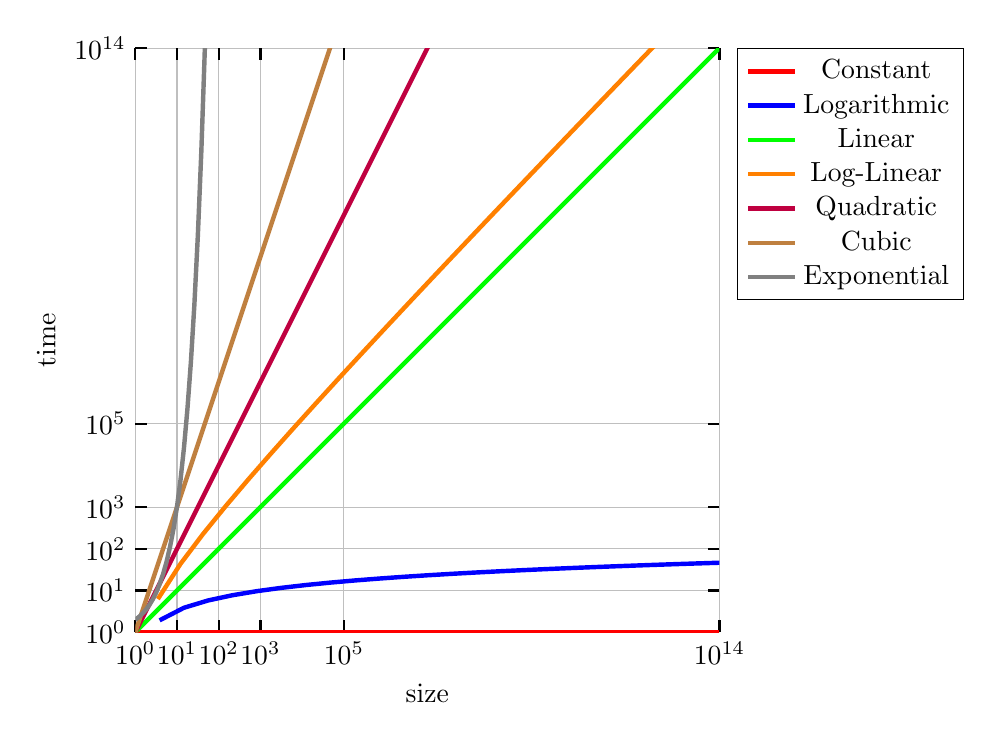
\begin{tikzpicture}
        \begin{loglogaxis}[ xlabel={size}, ylabel={time}, legend pos=outer north east, legend style={cells={align=left}}, xmin=1, xmax=100000000000000, ymin=1, ymax=100000000000000, grid=major, xtick={1,10,100,1000,100000,100000000000000}, ytick={1,10,100,1000,100000,100000000000000}, tick align=inside, minor tick num=4, axis line style={draw=none}, every tick/.style={thick}, width=9cm, height=9cm, axis equal]
            \addplot[domain=1:100000000000000,red,ultra thick] {1};
            \addlegendentry{Constant}
            \addplot[domain=1:100000000000000,blue,ultra thick] {log2(x)};
            \addlegendentry{Logarithmic}
            \addplot[domain=1:100000000000000,green,ultra thick] {x};
            \addlegendentry{Linear}
            \addplot[domain=1:10000000000000,orange,ultra thick] {x*log2(x)};
            \addlegendentry{Log-Linear}
            \addplot[domain=1:100000000000,purple,ultra thick] {x^2};
            \addlegendentry{Quadratic}
            \addplot[domain=1:100000,brown,ultra thick] {x^3};
            \addlegendentry{Cubic}
            \addplot[domain=1:100,gray,ultra thick] {2^x};
            \addlegendentry{Exponential}
        \end{loglogaxis}
        \end{tikzpicture}
\end{center}
\subsubsection*{Types of Analyses}
\begin{spacing}{1.5}
\begin{tabularx}{1\textwidth}{X|X|X}
    \hline
    \textbf{Best case - Lower bound} & \textbf{Worst case - Upper bound} & \textbf{Average case - Expected cost} \\
    \hline
    Big Omega ($\Omega()$)&Big Oh (O$()$)&Big Theta ($\Theta()$)\\
    \hline
    Determined by “easiest” input & Determined by “most difficult” input & Need a model for “random” input \\
    \hline
    Provides a goal for all inputs & Provides a guarantee for all inputs & Provides a way to predict performance \\
    \hline
\end{tabularx}
\end{spacing}
\subsection{Abstract Data Types (ADTs)}
\begin{itemize}
    \item Linear (Array, List, Stack, Queue, Set and Bag, Map, Priority Queue)
    \item Non-linear (Tree, Graph)
\end{itemize}
\begin{spacing}{1.5}
\begin{tabularx}{1\textwidth}{X|X|X}
    \hline
    \textbf{Array} & \textbf{List} & \textbf{Stack}\\
    \hline
    fixed number of items, indexable&dynamic number of items&A list that last-in, first-out\\
    \hline
    \verb|set(index, element)|&\verb|append(item)|&\verb|push (item)|\\
    \verb|get(index)|&\verb|prepend(item)|&\verb|pop()|\\
    &\verb|head()|&\verb|isEmpty()|\\
    &\verb|tail()|&\\
    \hline
\end{tabularx}
\ \\\ \\\ \\
\begin{tabularx}{1\textwidth}{X|p{0.64\textwidth}}
    \hline
    \textbf{Queue} & \textbf{Set and Bag}\\
    \hline
    A list that first-in, first-out&Set and Bag have unindexed, unordered elements. Set's element is unrepeated. Bag's element is possibly duplicated\\
    \hline
    \verb|enqueue (item)|&\verb|insert (item)|\\
    \verb|dequeue()|&\verb|remove(item)|\\
    \verb|head()|&\verb|contains(item)|\\
    \hline
\end{tabularx}
\ \\\ \\\ \\
\begin{tabularx}{1\textwidth}{X|X}
    \hline
    \textbf{Map} & \textbf{Priority Queue}\\
    \hline
    A list that can hold data in (key, value) pairs. Keys are unique, and can only hold one value & A queue where items are inserted/removed based on a given priority\\
    \hline
    \verb|insert (key, value)|&\verb|enqueue(item, priority)|\\
    \verb|remove(key)|&\verb|dequeue()|\\
    \verb|update(key, value)|&\\
    \verb|lookup(key)|&\\
    \hline
\end{tabularx}
\end{spacing}
\subsubsection*{ADTs and Data Structures}
\begin{spacing}{1.5}
\begin{tabularx}{1\textwidth}{X|p{0.6\textwidth}}
    \hline
    \textbf{ADTs} & \textbf{Common Implementations (Data Structures)}\\
    \hline
    Array&array\\
    List&array, linked list\\
    Queue&array, linked list\\
    Stack&array, linked list\\
    Set and Bag&hash table\\
    Map&hash table\\
    Priority Queue&heap\\
    \hline
\end{tabularx}
\end{spacing}


\section{Sort Algorithms}
\subsection{Elementary Sorts}
\subsubsection*{Selection Sort}
Key idea:
\begin{enumerate}
    \item scan array from left to right
    \item in iteration \verb|i|, find the index \verb|min| of the smallest remaining entry in the array
    \item swap \verb|a[i]| and \verb|a[min]|
\end{enumerate}
\begin{lstlisting}
def selectionSort(xs: list) -> None:
for i in range(len(xs)):
    min = i
    j = i+1
    while j < len(xs):
        if xs[j] < xs[min]:
            min = j
        j += 1
    if min != i:
        xs[i], xs[min] = xs[min], xs[i]
    i += 1
\end{lstlisting}
\begin{spacing}{1.5}
\begin{tabularx}{1\textwidth}{|X|X|X|}
    \hline
    \textbf{Best case} & \textbf{Worst case} & \textbf{Average case}\\
    \hline
    $N^2$&$N^2$&$N^2$\\
    \hline
\end{tabularx}
\end{spacing}
\subsubsection*{Insert Sort}
Key idea:
\begin{itemize}
    \item scan array from left to right
    \item in iteration i, swap a[i] with each larger entry to its left
\end{itemize}
\begin{lstlisting}
def insertSort(xs: list) -> None:
for i in range(len(xs)):
    j = i
    while j > 0:
        if xs[j] < xs[j-1]:
            xs[j], xs[j-1] = xs[j-1], xs[j]
        j -= 1
\end{lstlisting}
\begin{spacing}{1.5}
\begin{tabularx}{1\textwidth}{|X|X|X|}
    \hline
    \textbf{Best case} & \textbf{Worst case} & \textbf{Average case}\\
    \hline
    $N$&$N^2$&$N^2$\\
    \hline
\end{tabularx}
\end{spacing}

\subsection{Merge Sort}
\subsubsection*{Key idea - Divide and conquer}
\begin{itemize}
    \item Divide an array in two halves
    \item Sort each half separately
    \item Merge the two halves
\end{itemize}
\subsubsection*{Pseudocode}
\begin{lstlisting}
def merge(xs: list, aux: list, lo: int, mid: int, hi: int) -> None:
    k = lo
    while k <= hi:
        aux[k] = xs[k]
        k += 1

    i, j, k = lo, mid+1, lo
    while k <= hi:
        if i > mid:
            xs[k], j, k = aux[j], j+1, k+1
        elif j > hi:
            xs[k], i, k = aux[i], i+1, k+1
        elif aux[j] < aux[i]:
            xs[k], j, k = aux[j], j+1, k+1
        else:
            xs[k], i, k = aux[i], i+1, k+1


def sort(xs: list, aux: list, lo: int, hi: int) -> None:
    if hi <= lo:
        return

    mid = lo + (hi-lo)//2

    sort(xs, aux, lo, mid)
    sort(xs, aux, mid+1, hi)
    merge(xs, aux, lo, mid, hi)
\end{lstlisting}
\begin{spacing}{1.5}
\begin{tabularx}{1\textwidth}{|X|X|X|}
    \hline
    \textbf{Best case} & \textbf{Worst case} & \textbf{Average case}\\
    \hline
    $N\,\lg\,N$&$N\,\lg\,N$&$N\,\lg\,N$\\
    \hline
\end{tabularx}
\end{spacing}
\subsubsection*{Divide and Sort Steps}
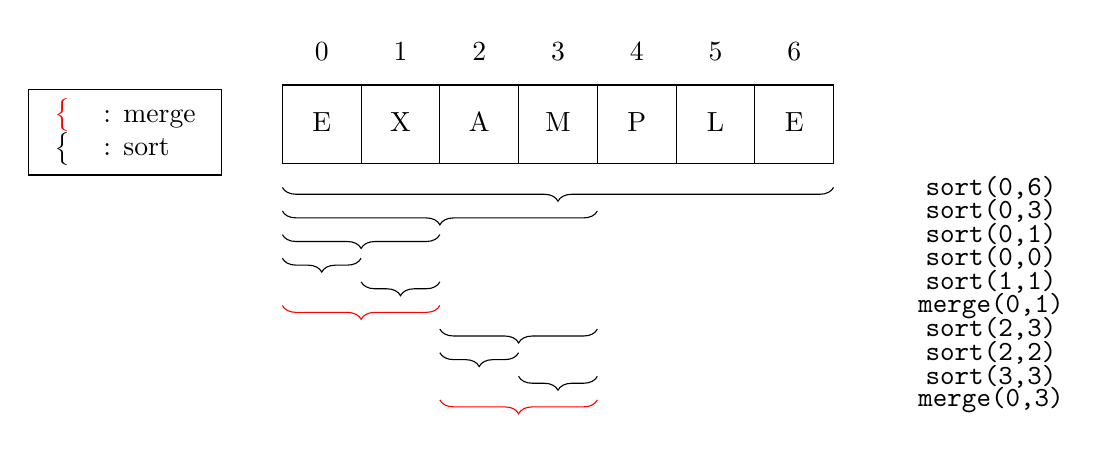
\begin{tikzpicture}[node distance=1cm]
% draw array
\draw (0,0) grid (7,1);
\foreach \i/\n in {0/E,1/X,2/A,3/M,4/P,5/L,6/E} {
\node at (\i+0.5,0.5) {\strut \n};
\node at (\i+0.5,1.4) {\strut \i};
}
% draw braces
\draw [decorate,decoration={brace,amplitude=5pt,mirror}] (0,-0.3) -- (7,-0.3);
\node at (9,-0.3) {\verb|sort(0,6)|};
\draw [decorate,decoration={brace,amplitude=5pt,mirror}] (0,-0.6) -- (4,-0.6);
\node at (9,-0.6) {\verb|sort(0,3)|};
\draw [decorate,decoration={brace,amplitude=5pt,mirror}] (0,-0.9) -- (2,-0.9);
\node at (9,-0.9) {\verb|sort(0,1)|};
\draw [decorate,decoration={brace,amplitude=5pt,mirror}] (0,-1.2) -- (1,-1.2);
\node at (9,-1.2) {\verb|sort(0,0)|};
\draw [decorate,decoration={brace,amplitude=5pt,mirror}] (1,-1.5) -- (2,-1.5);
\node at (9,-1.5) {\verb|sort(1,1)|};
\draw [decorate,decoration={brace,amplitude=5pt,mirror,},color=red] (0,-1.8) -- (2,-1.8);
\node at (9,-1.8) {\verb|merge(0,1)|};
\draw [decorate,decoration={brace,amplitude=5pt,mirror}] (2,-2.1) -- (4,-2.1);
\node at (9,-2.1) {\verb|sort(2,3)|};
\draw [decorate,decoration={brace,amplitude=5pt,mirror}] (2,-2.4) -- (3,-2.4);
\node at (9,-2.4) {\verb|sort(2,2)|};
\draw [decorate,decoration={brace,amplitude=5pt,mirror}] (3,-2.7) -- (4,-2.7);
\node at (9,-2.7) {\verb|sort(3,3)|};
\draw [decorate,decoration={brace,amplitude=5pt,mirror},color=red] (2,-3) -- (4,-3);
\node at (9,-3) {\verb|merge(0,3)|};
% Add annotation on the right
\node[rectangle, draw] at (-2,0.4) {
\begin{tabular}{rl}
    \textcolor{red}{\big\{} &: merge \\
    \textcolor{black}{\big\{} &: sort
\end{tabular}
};
\end{tikzpicture}


\subsection{Quick Sort}
\subsubsection*{Key idea}
\begin{itemize}
    \item Shuffle the array \verb|a[]|
    \item Partition \verb|a[]| so that, for some \verb|j|
    \begin{itemize}
        \item Entry \verb|a[j]| is in place
        \item \verb|a[i]<=a[j]| for any \verb|i<j|
        \item \verb|a[i]>=a[j]| for any \verb|i>j|
    \end{itemize}
    \item Sort each partition recursively
\end{itemize}

\subsubsection*{Pseudocode}
\begin{lstlisting}
def partition(xs: list, lo: int, hi: int) -> int:
    i, j, pivot = lo, hi + 1, xs[lo]
    while True:
        i, j = i + 1, j - 1
        while xs[i] < pivot:
            i += 1
            if i == hi:
                break
        while pivot < xs[j]:
            j -= 1
            if j == lo:
                break
        if i >= j:
            break
        xs[i], xs[j] = xs[j], xs[i]
    xs[lo], xs[j] = xs[j], xs[lo]
    return j


def sort(xs: list, lo: int, hi: int) -> None:
    if hi <= lo:
        return
    j = partition(xs, lo, hi)
    sort(xs, lo, j - 1)
    sort(xs, j + 1, hi)
\end{lstlisting}
\begin{spacing}{1.5}
\begin{tabularx}{1\textwidth}{|X|X|X|}
    \hline
    \textbf{Best case} & \textbf{Worst case} & \textbf{Average case}\\
    \hline
    $N^2$&$N\,\lg\,N$&$N\,\lg\,N$\\
    \hline
\end{tabularx}
\end{spacing}

\subsubsection*{Practical Improvements}
\begin{itemize}
    \item Use insertion sort on small subarrays (<10 items)
    \item Best choice pivot = median value (e.g., median of 3 random items)
\end{itemize}

\subsubsection*{Some Properties}
\begin{itemize}
    \item Quick sort running time on duplicate keys could be quadratic
\end{itemize}

\subsection{Heap Sort}
\subsubsection*{Binary Heap Data Structure}
\begin{lstlisting}
class MaxPriorityQueue:
    def __init__(self) -> None:
        self.heap = [None]
        self.tail = 0

    def enqueue(self, key) -> None:
        self.heap.append(key)
        self.tail += 1
        self._swim(self.tail)

    def dequeue(self):
        if self.tail == 0:
            return None
        max = self.heap[1]
        self.heap[1], self.heap[self.tail] = self.heap[self.tail], self.heap[1]
        self.heap[self.tail] = None
        self.tail -= 1
        self._sink(1)
        self.heap.pop()
        return max

    def _swim(self, i: int) -> None:
        while i > 1 and self.heap[i//2] < self.heap[i]:
            self.heap[i], self.heap[i//2] = self.heap[i//2], self.heap[i]
            i //= 2

    def _sink(self, i: int) -> None:
        while 2*i <= self.tail:
            j = 2*i
            if j < self.tail and self.heap[j] < self.heap[j+1]:
                j += 1
            if self.heap[i] >= self.heap[j]:
                break
            self.heap[i], self.heap[j] = self.heap[j], self.heap[i]
            i = j
\end{lstlisting}
\begin{spacing}{1.5}
\begin{tabularx}{1\textwidth}{|p{0.2\textwidth}|X|X|X|}
    \hline
    &\textbf{Best case} & \textbf{Worst case} & \textbf{Average case}\\
    \hline
    \textbf{enqueue}&$1$&$\log N$&$\log N$\\
    \hline
    \textbf{dequeue}&$\log N$&$\log N$&$\log N$\\
    \hline
\end{tabularx}
\end{spacing}

\subsubsection*{Heap Sort}
Key idea:
\begin{itemize}
    \item Create a max-heap ordered array with all N keys
    \item Repeatedly remove the maximum key remaining
\end{itemize}
\begin{lstlisting}
def sink(xs: list, i: int, tail: int) -> None:
    while 2*i <= tail:
        j = 2*i
        if j < tail and xs[j] < xs[j+1]:
            j += 1
        if xs[i] >= xs[j]:
            break
        xs[i], xs[j] = xs[j], xs[i]
        i = j


def heapSort(xs: list) -> None:
    k = len(xs)//2
    while k >= 1:
        sink(xs, k, len(xs)-1)
        k -= 1
    n = len(xs)-1
    while n > 1:
        xs[1], xs[n] = xs[n], xs[1]
        n -= 1
        sink(xs, 1, n)

#The index of the heap starts from 1, therefore a dummy element is added to the beginning of the list.
test = [None]+[5, 9, 54, 11, 3, 6, 2, -7, -3, -9, 4, 8, -6]
heapSort(test)
print(test)
\end{lstlisting}
\begin{spacing}{1.5}
\begin{tabularx}{1\textwidth}{|X|X|X|}
    \hline
    \textbf{Best case} & \textbf{Worst case} & \textbf{Average case}\\
    \hline
    $N\,\lg\,N$&$N\,\lg\,N$&$N\,\lg\,N$\\
    \hline
\end{tabularx}
\end{spacing}

\subsection{Summary}
\begin{spacing}{1.5}
\begin{tabularx}{1\textwidth}{|X|X|X|X|X|X|}
    \hline
    &\textbf{In place} & \textbf{Stable} & \textbf{Worst} & \textbf{Average case} & \textbf{Best case}\\
    \hline
    \textbf{Selection}&\centering\checkmark&&$N^2$&$N^2$&$N^2$\\
    \hline
    \textbf{Insertion}&\centering\checkmark&\centering\checkmark&$N^2$&$N^2$&$N$\\
    \hline
    \textbf{Merge-sort}&&\centering\checkmark&$N\,\lg\,N$&$N\,\lg\,N$&$N\,\lg\,N$\\
    \hline
    \textbf{Quick-sort}&\centering\checkmark&&$N^2$&$N\,\lg\,N$&$N\,\lg\,N$\\
    \hline
    \textbf{Heapsort}&\centering\checkmark&&$N\,\lg\,N$&$N\,\lg\,N$&$N\,\lg\,N$\\
    \hline
\end{tabularx}
\end{spacing}
\begin{itemize}
    \item An in-place sorting algorithm is one that does not require additional memory to be allocated for temporary storage during the sorting process
    \item A sorting algorithm is said to be stable if two items with equal keys appear in the same order in the sorted output as they appear in the input array
\end{itemize}



\section{Search Algorithms}
\subsection{Symbol Table}
\begin{spacing}{1.5}
\begin{tabularx}{1\textwidth}{X}
    \hline
    \textbf{Symbol Table} \\
    \hline
    Abstract data type to handle key-value pairs\\
    \hline
    \verb|put(key, value)|\\
    \verb|get(key)|\\
    \hline
\end{tabularx}
\end{spacing}

\subsubsection*{Common assumptions}
\begin{itemize}
    \item Keys are unique
    \item Values are not null
    \item Keys have a total order relation:
    \begin{itemize}
        \item Antisymmetry: if $a\leq b$ and $b\leq a$, then $a=b$
        \item Transitivity: if $a\leq b$ and $b\leq c$, then $a\leq c$
        \item Totality: either $a\leq b$ or $b\leq a$
    \end{itemize}
\end{itemize}

\subsection{Binary Search Tree}
A binary search tree is a binary tree in symmetric order
\begin{itemize}
    \item A binary tree is in symmetric order if each node has a key, and every node's key is:
    \begin{itemize}
        \item Larger than all keys in its left subtree
        \item Smaller than all keys in its right subtree
    \end{itemize}
\end{itemize}

\subsubsection*{Pseudocode}
\begin{lstlisting}
class Node:
    def __init__(self, key, value) -> None:
        self.key = key
        self.value = value
        self.left = None
        self.right = None

    def get(self, key):
        if self.key == key:
            return self.value
        elif key < self.key and self.left:
            return self.left.get(key)
        elif key > self.key and self.right:
            return self.right.get(key)
        else:
            return None
        
    def put(self, key, value):
        if key == self.key:
            self.value = value
        elif key < self.key:
            if self.left is None:
                self.left = Node(key, value)
            else:
                self.left.put(key, value)
        elif key > self.key:
            if self.right is None:
                self.right = Node(key,value)
            else:
                self.right.put(key,value)
\end{lstlisting}
\begin{lstlisting}
from BSTNode import BSTNode

class BSTree:
    def __init__(self) -> None:
        self.root = None
    
    def get(self, key):
        if self.root is None:
            return None
        else:
            return self.root.get(key)
        
    def put(self, key, value):
        if self.root is None:
            self.root = BSTNode(key,value)
        else:
            self.root.put(key, value)
\end{lstlisting}

\subsection{BST Additional Operations}
\subsubsection*{Min and Max}
\begin{lstlisting}
class BSTNode:
    def min(self):
        if self.left is None:
            return self.key
        else:
            return self.left.min()
        
    def max(self):
        if self.right is None:
            return self.key
        else:
            return self.right.max()
\end{lstlisting}
\begin{lstlisting}
class BSTree:
    def min(self):
        if self.root is None:
            return None
        else:
            return self.root.min()

    def max(self):
        if self.root is None:
            return None
        else:
            return self.root.max()
\end{lstlisting}

\subsection*{Floor and Ceiling}
\begin{lstlisting}
class BSTNode:
    def floor(self, key):
        if key == self.key:
            return self.key
        elif key < self.key:
            if self.left is None:
                return None
            else:
                return self.left.floor(key)
        else:
            if self.right is None:
                return self.key
            else:
                right_floor = self.right.floor(key)
                return right_floor if right_floor is not None else self.key
            
    def ceiling(self, key):
        if key == self.key:
            return self.key
        elif key > self.key:
            if self.right is None:
                return None
            else:
                return self.right.ceiling(key)
        else:
            if self.left is None:
                return self.key
            else:
                left_ceiling = self.left.ceiling(key)
                return left_ceiling if left_ceiling is not None else self.key
\end{lstlisting}
\begin{lstlisting}
class BSTree:
    def floor(self, key):
        if self.root is None:
            return None
        else:
            return self.root.floor(key)
        
    def ceiling(self, key):
        if self.root is None:
            return None
        else:
            return self.root.ceiling(key)
\end{lstlisting}
\subsubsection*{Delete}
\begin{lstlisting}
class BSTNode:
    def delete(self, key):
        if self is None:
            return None
        if key < self.key:
            self.left = self.left.delete(key)
        elif key > self.key:
            self.right = self.right.delete(key)
        else:
            if self.left is None:
                return self.right
            if self.right is None:
                return self.left
            temp = self
            self = min(self.right)
            self.right = temp.right._deleteMin()
            self.left = temp.left
        return self

            
    def _deleteMin(self):
        if self.left is None:
            return self.right
        self.left = self.left._deleteMin()
        return self
\end{lstlisting}
\begin{lstlisting}
class BSTree:
    def delete(self, key):
        if self.root is None:
            return None
        else:
            self.root = self.root.delete(key)
\end{lstlisting}
\begin{spacing}{1.5}
\begin{tabularx}{1\textwidth}{|X|X|X|X|X|X|}
    \hline
    \multicolumn{3}{|c|}{\textbf{Worst Case}} &\multicolumn{3}{c|}{\textbf{Average Case}}\\
    \hline
    \textbf{Search} & \textbf{Insert} & \textbf{Delete} & \textbf{Search (hit)} & \textbf{Insert} & \textbf{Search}\\
    \hline
    $N$&$N$&$N$&$c\,\lg\,N$&$c\,\lg\,N$&$\sqrt{N}$\\
    \hline
\end{tabularx}
\end{spacing}

\begin{spacing}{1.5}
\begin{tabularx}{1\textwidth}{|X|X|X|X|}
    \hline
    \textbf{Get} & \textbf{Put} & \textbf{Min/max} & \textbf{Floor/ceiling}\\
    \hline
    $h\sim \lg\,N$&$h\sim \lg\,N$&$h\sim \lg\,N$&$h\sim \lg\,N$\\
    \hline
    \textbf{Delete} & \textbf{Ordering iteration}&&\\
    \hline
    $h\sim \lg\,N$&$N$&&\\
    \hline
\end{tabularx}
\end{spacing}

\subsection{Balanced Search Tree}
\subsubsection*{Two Three Search Tree}
A 2-3 search tree is a tree where each node can be of two types:
\begin{itemize}
    \item 2-node: one key, two children
    \item 3-node: two keys, three children
\end{itemize}

\subsubsection*{Feature}
\begin{itemize}
    \item Symmetric order. In-order traversal yields keys in ascending order
    \item Perfect balance. Every path from the root to a null link has the same length
\end{itemize}

\subsubsection*{Insert operation - put (new key)}
\begin{itemize}
    \item Case 1: insert the new key in a 2-node
    \begin{itemize}
        \item Transform the 2-node into a 3-node
    \end{itemize}
    \item Case 2: insert the new key in a 3-node
    \begin{itemize}
        \item Add the new key to a 3-node to create a temporary 4-node
        \item Move the middle key of the 4-node into its parent node and create two 2-nodes children
        \item Repeat up the tree as necessary
        \item If you reach the root and it is a 4-node, split it into three 2-nodes.
    \end{itemize}
\end{itemize}

\subsubsection*{Graph Example}
\begin{center}
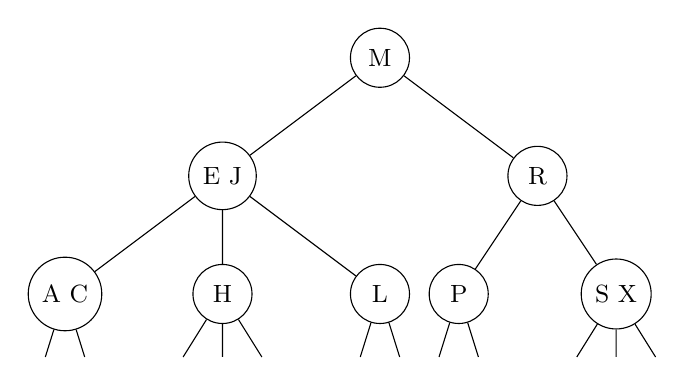
\begin{tikzpicture}[
    level 1/.style={sibling distance=4cm},
    level 2/.style={sibling distance=2cm},
    level 3/.style={sibling distance=0.5cm, level distance=0.8cm},
    every node/.style = {
        draw, circle, minimum size=0.75cm, font=\small
    }
]
\node {M}
    child {
        node {E J}
        child {
            node {A C}
            child {}
            child {}
        }
        child {
            node {H}
            child {}
            child {}
            child {}
        }
        child {
            node {L}
            child {}
            child {}
        }
    }
    child {
        node {R}
        child {
            node {P}
            child {}
            child {}
        }
        child {
            node {S X}
            child {}
            child {}
            child {}
        }
    };
\end{tikzpicture}
\end{center}

\begin{spacing}{1.5}
\begin{tabularx}{1\textwidth}{|X|X|X|X|X|X|}
    \hline
    \multicolumn{3}{|c|}{\textbf{Worst Case}} &\multicolumn{3}{c|}{\textbf{Average Case}}\\
    \hline
    \textbf{Search} & \textbf{Insert} & \textbf{Delete} & \textbf{Search (hit)} & \textbf{Insert} & \textbf{Search}\\
    \hline
    $c\,\lg\,N$&$c\,\lg\,N$&$c\,\lg\,N$&$c\,\lg\,N$&$c\,\lg\,N$&$c\,\lg\,N$\\
    \hline
\end{tabularx}
\end{spacing}

\subsubsection*{Red Black Tree}
Key idea: represent a 2-3 Tree as a BST\\
How: transform a 3-node into a left-leaning BST (two 2-nodes connected by an ”internal” red link)\\
\newline
Definition of a left-leaning red-black (LLRB) BST: a BST such that
\begin{itemize}
    \item Every path from the root to null links has the same number of black links (perfect black balance)
    \item No node has 2 red links connected to it (or else that would be a 4-node)
    \item Red links lean left
\end{itemize}

\subsubsection*{Same Example}
\begin{center}
    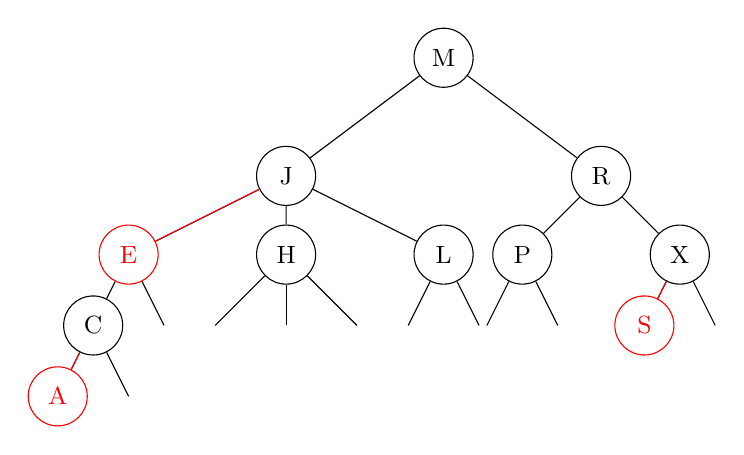
\begin{tikzpicture}[
        level 1/.style={sibling distance=4cm},
        level 2/.style={sibling distance=2cm, level distance=1cm},
        level 3/.style={sibling distance=0.9cm, level distance=0.9cm},
        level 4/.style={sibling distance=0.9cm, level distance=0.9cm},
        every node/.style = {
        draw, circle, minimum size=0.75cm, font=\small
        }
        ]
        \node {M}
        child {
            node (J) {J}
            child {
                node[red] (E) {E}
                child {
                    node (C) {C}
                    child {node[red] (A) {A}}
                    child {}
                }
                child {}
            }
            child {
                node {H}
                child {}
                child {}
                child {}
            }
            child {
                node {L}
                child {}
                child {}
            }
        }
        child {
            node {R}
            child {
                node {P}
                child {}
                child {}
            }
            child {
                node (X) {X}
                child {node[red] (S) {S}}
                child {}
            }
        };

        \draw[red] (J) -- (E);
        \draw[red] (C) -- (A);
        \draw[red] (X) -- (S);
    \end{tikzpicture}
\end{center}

\subsubsection*{Pseudocode}
\begin{lstlisting}
class LLRBNode:
    def __init__(self, key, value) -> None:
        self.key = key
        self.value = value
        self.left = None
        self.right = None
        self.color = False  # True for red and False for black

    def get(self, key):
        if self.key == key:
            return self.value
        elif key < self.key and self.left:
            return self.left.get(key)
        elif key > self.key and self.right:
            return self.right.get(key)
        else:
            return None
\end{lstlisting}

\begin{lstlisting}
from LLRBNode import LLRBNode

class LLRBTre:
    def __init__(self) -> None:
        self.root = None

    def get(self, key):
        if self.root is None:
            return None
        else:
            return self.root.get(key)

    def put(self, key, value):
        if self.root is None:
            self.root = LLRBNode(key, value)
        else:
            self.root = self._put(self.root, key, value)

    def _put(self, n: LLRBNode, key, value) -> LLRBNode:
        if n is None:
            return LLRBNode(key, value)
        if key == n.key:
            n.value = value
        elif key < n.key:
            n.left = self._put(n.left, key, value)
        else:
            n.right = self._put(n.right, key, value)

        if self._isRed(n) and not self._isRed(n.left):
            n = self._left_rotation(n)
        if self._isRed(n.left) and self._isRed(n.left.left):
            n = self._right_rotation(n)
        if self._isRed(n.left) and self._isRed(n.right):
            self._color_flip(n)
        return n

    def _isRed(self, n: LLRBNode) -> bool:
        if n is None:
            return False
        return n.color

    def _left_rotation(self, n: LLRBNode) -> LLRBNode:
        x = n.right
        n.right = x.left
        x.left = n
        x.color = n.color
        n.color = True
        return x

    def _right_rotation(self, n: LLRBNode) -> LLRBNode:
        x = n.left
        n.left = x.right
        x.right = n
        x.color = n.color
        n.color = True
        return x

    def _color_flip(self, n: LLRBNode):
        n.color = True
        n.left.color = False
        n.right.color = False
\end{lstlisting}
\begin{spacing}{1.5}
\begin{tabularx}{1\textwidth}{|X|X|X|X|X|X|}
    \hline
    \multicolumn{3}{|c|}{\textbf{Worst Case}} &\multicolumn{3}{c|}{\textbf{Average Case}}\\
    \hline
    \textbf{Search} & \textbf{Insert} & \textbf{Delete} & \textbf{Search (hit)} & \textbf{Insert} & \textbf{Search}\\
    \hline
    $2\,\lg\,N$&$2\,\lg\,N$&$2\,\lg\,N$&$1\,\lg\,N$&$1\,\lg\,N$&$1\,\lg\,N$\\
    \hline
\end{tabularx}
\end{spacing}

\subsection{Hash Tables}
If our keys are simple, such as primitive data type, integer or strings, then we can use a hash table to store and retrieve data efficiently. Hash tables can only efficiently perform insertion and search operations, but cannot sort or perform sequential traversal operations.\\
\newline
Key idea: reduce the symbol table ADT into an array ADT\\
How: use a hash function to transform keys to integers used as indexes in an array where the corresponding values are

\subsubsection*{Hash Function}
Properties: scramble keys to produce an index in [0,M] so that:
\begin{itemize}
    \item The mapping is deterministic
    \item The mapping can be computed very fast
    \item The probability of collisions is very low
\end{itemize}
\begin{center}
    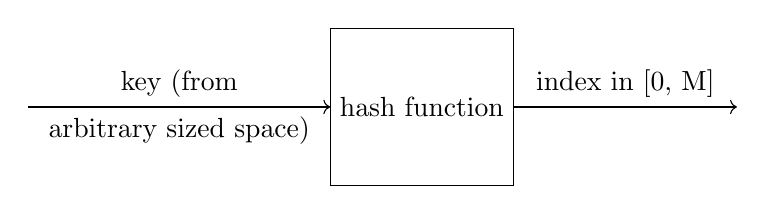
\begin{tikzpicture}
        % nodes
        \node[draw, rectangle, minimum width=2cm, minimum height=2cm] (hash) at (4,0) {hash function};
        % arrows
        \draw[->] (-1,0) -- node[above]{key (from }node[below]{arbitrary sized space)} (hash.west);
        \draw[->] (hash.east) -- node[above]{index in [0, M]} (8,0);
    \end{tikzpicture}
\end{center}
\begin{lstlisting}
def simpleHash(s: str, M: int) -> int:
    hash = 0
    P = 31
    for i in range(len(s)):
        hash = (P * hash + ord(s[i]))
    return hash % M
\end{lstlisting}

\subsubsection*{Separate Chaining}
Data structure: array of $M(<N)$ linked lists\\
Operations
\begin{itemize}
    \item Hash $<$key$>$: map key to integer $i$ in $[0, M-1]$
    \item Insert $<$key, value$>$: put value at the front of $i$th chain (if not already there)
    \item Search $<$key$>$: linearly scan the ith chain
\end{itemize}

How to choose $M$
\begin{itemize}
    \item $M$ too large $\to$ space waste (too many empty chains)
    \item $M$ too small $\to$ search time blows up (chains too long)
    \item $M\approx N/5$
\end{itemize}

\begin{lstlisting}
class Node:
    def __init__(self, key, value) -> None:
        self.key = key
        self.value = value
        self.next = None
\end{lstlisting}

\begin{lstlisting}
from Node import Node

class SeparateChainingHashTable:
    def __init__(self, n: int):
        self.m = n // 5
        self.table = [None] * self.m

    def get(self, key):
        index = hash(key) % self.m
        current = self.table[index]
        while current is not None:
            if current.key == key:
                return current.value
            current = current.next
        return None

    def put(self, key, value):
        index = hash(key) % self.m
        current = self.table[index]
        if current is None:
            self.table[index] = Node(key, value)
            return
        while current is not None:
            if current.key == key:
                current.value = value
                return
            if current.next is None:
                current.next = Node(key, value)
                return
            current = current.next
\end{lstlisting}

\begin{spacing}{1.5}
\begin{tabularx}{1\textwidth}{|X|X|X|X|X|X|}
    \hline
    \multicolumn{3}{|c|}{\textbf{Worst Case}} &\multicolumn{3}{c|}{\textbf{Average Case}}\\
    \hline
    \textbf{Search} & \textbf{Insert} & \textbf{Delete} & \textbf{Search (hit)} & \textbf{Insert} & \textbf{Search}\\
    \hline
    $\lg\,N$&$\lg\,N$&$\lg\,N$&$3-5$&$3-5$&$3-5$\\
    \hline
\end{tabularx}
\end{spacing}

\subsubsection*{Linear Probing}
Data structure: two arrays of size M $>$ N (one for keys, one for values)\\
Operations
\begin{itemize}
    \item Hash $<$key$>$: map key to integer $i$ in $[0, M-1]$
    \item Insert $<$key, value$>$: put value at index $i$ if available, or else try $i+1, i+2$, etc.
    \item Search $<$key$>$: access table index $i$; if occupied but no match, try $i+1, i+2$, etc.
\end{itemize}
How to choose M
\begin{itemize}
    \item $M$ too large $\to$ space waste (too many empty array entries)
    \item $M$ too small $\to$ search time blows up
    \item $M\approx 2\times N$
\end{itemize}

\begin{lstlisting}
class LinearProbingHashTable:
    def __init__(self, n: int) -> None:
        self.m = n * 2 + 1
        self.key_table = [None] * self.m
        self.value_table = [None] * self.m

    def get(self, key):
        index = hash(key) % self.m
        while self.key_table[index] is not None:
            if self.key_table[index] == key:
                return self.value_table[index]
            index = (index + 1) % self.m
        return None

    def put(self, key, value):
        index = hash(key) % self.m
        while self.key_table[index] is not None:
            if self.key_table[index] == key:
                self.value_table[index] = value
                return
            index = (index + 1) % self.m
        self.key_table[index] = key
        self.value_table[index] = value
\end{lstlisting}

\begin{spacing}{1.5}
\begin{tabularx}{1\textwidth}{|X|X|X|X|X|X|}
    \hline
    \multicolumn{3}{|c|}{\textbf{Worst Case}} &\multicolumn{3}{c|}{\textbf{Average Case}}\\
    \hline
    \textbf{Search} & \textbf{Insert} & \textbf{Delete} & \textbf{Search (hit)} & \textbf{Insert} & \textbf{Search}\\
    \hline
    $N$&$N$&$N$&$3-5$&$3-5$&$3-5$\\
    \hline
\end{tabularx}
\end{spacing}

\subsection{Summary}
\begin{spacing}{1.5}
\begin{tabularx}{1\textwidth}{|X|X|X|X|X|X|X|}
    \hline
    & \multicolumn{3}{c|}{\textbf{Worst Case}} &\multicolumn{3}{c|}{\textbf{Average Case}}\\
    \hline
    & \textbf{Search} & \textbf{Insert} & \textbf{Delete} & \textbf{Search (hit)} & \textbf{Insert} & \textbf{Search}\\
    \hline
    \textbf{BST}&$N$&$N$&$N$&$c\,\lg\,N$&$c\,\lg\,N$&$\sqrt{N}$\\
    \hline
    \textbf{2-3 Search Tree}&$c\,\lg\,N$&$c\,\lg\,N$&$c\,\lg\,N$&$c\,\lg\,N$&$c\,\lg\,N$&$c\,\lg\,N$\\
    \hline
    \textbf{LLRB BST}&$2\,\lg\,N$&$2\,\lg\,N$&$2\,\lg\,N$&$1\,\lg\,N$&$1\,\lg\,N$&$1\,\lg\,N$\\
    \hline
    \textbf{Separate Chaining}&$\lg\,N$&$\lg\,N$&$\lg\,N$&$3-5$&$3-5$&$3-5$\\
    \hline
    \textbf{Linear Probing}&$N$&$N$&$N$&$3-5$&$3-5$&$3-5$\\
    \hline
\end{tabularx}
\end{spacing}

\section{Graph Algorithms}
\subsection{Undirected Graphs}
\subsubsection*{Terminology}
\begin{itemize}
    \item Degree. Number of edges that are incident to the vertex.
    \item Path. Sequence of vertices connected by edges.
    \item Cycle. Path whose first and last vertices are the same.
    \item Connected Component. Set of vertices connected to each other.
\end{itemize}

\begin{center}
    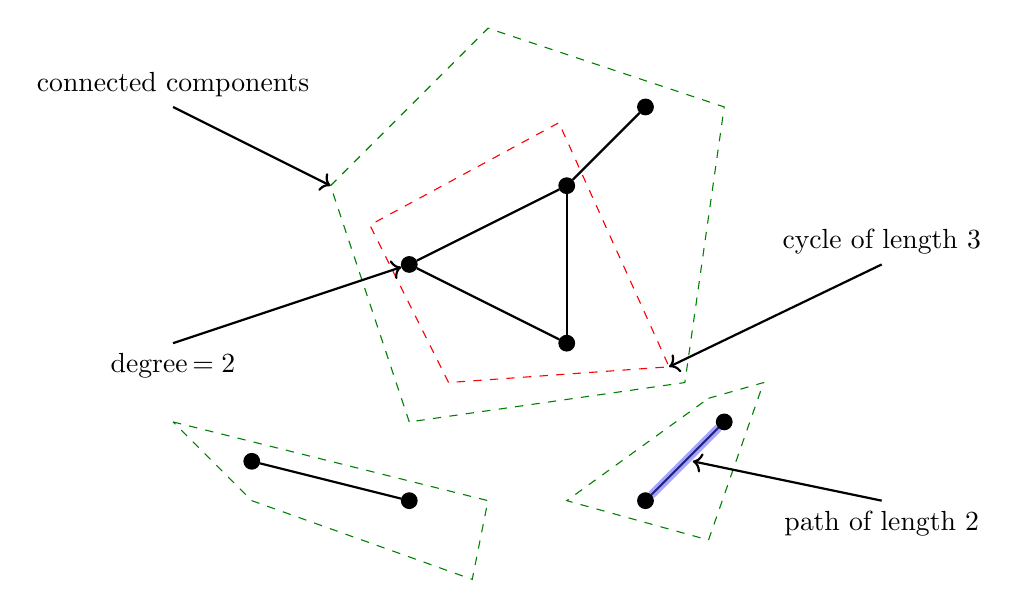
\begin{tikzpicture}[node distance=2cm, every edge/.style={draw=black,very thick}]
    % nodes
    \node[circle,draw,fill=black,inner sep=2pt] (v1) at(0,0) {};
    \node[circle,draw,fill=black,inner sep=2pt] (v2) at(0,3) {};
    \node[circle,draw,fill=black,inner sep=2pt] (v3) at(2,2) {};
    \node[circle,draw,fill=black,inner sep=2pt] (v4) at(3,0) {};
    \node[circle,draw,fill=black,inner sep=2pt] (v5) at(2,4) {};
    \node[circle,draw,fill=black,inner sep=2pt] (v6) at(3,5) {};
    \node[circle,draw,fill=black,inner sep=2pt] (v7) at(4,1) {};
    \node[circle,draw,fill=black,inner sep=2pt] (v8) at(-2,0.5) {};
    % degree
    \draw[thick] (v1) -- (v8);
    \draw[thick] (v2) -- (v3);
    \draw[thick] (v3) -- (v5);
    \draw[thick] (v6) -- (v5);
    \draw[thick] (v2) -- (v5);
    \draw[thick] (v7) -- (v4);
    \draw[line width=3pt, blue!70!white, opacity=0.5] (v7) -- (v4);

    \draw[dashed,green!50!black] (0,1) -- (-1,4) -- (1,6) -- (4,5) -- (3.5,1.5) -- (0,1);
    \draw[dashed,green!50!black] (-3,1) -- (1,0) -- (0.8,-1) -- (-2,0) -- (-3,1);
    \draw[dashed,green!50!black] (3.8,1.3) -- (4.5,1.5) -- (3.8,-0.5) -- (2,0) -- (3.8,1.3);

    \draw[dashed,red] (0.5,1.5) -- (-0.5,3.5) -- (1.9,4.8) -- (3.3,1.7) -- (0.5,1.5);

    \draw[->,thick] (-3,2)node[below]{degree$\,=2$} -- (v2);
    \draw[->,thick] (-3,5)node[above]{connected components} -- (-1,4);
    \draw[->,thick] (6,3)node[above]{cycle of length 3} -- (3.3,1.7);
    \draw[->,thick] (6,0)node[below]{path of length 2} -- (3.6,0.5);
    \end{tikzpicture}
\end{center}

\begin{lstlisting}
    class Graph:
        def __init__(self, num_vertices: int):
            self.num_vertices = num_vertices
            self.adj_list = [[] for _ in range(num_vertices)]
    
        def get_num_vertices(self) -> int:
            return self.num_vertices
    
        def add_edge(self, v: int, w: int) -> None:
            self.adj_list[v].append(w)
            self.adj_list[w].append(v)
    
        def get_adj_list(self, v: int) -> list:
            return self.adj_list[v]
    \end{lstlisting}

\subsubsection*{Depth-First Search}
Challenge: Find all vertices $v$ connected to $s$ (and their paths back to $s$)\\
How: To visit DFS a vertex $v$:
\begin{itemize}
    \item Mark vertex $v$ as visited
    \item Recursively visit all unmarked vertices $w$ adjacent to $v$
    \item Return (retrace steps) when no unvisited options left
\end{itemize}

\begin{lstlisting}
class Stack:
    def __init__(self) -> None:
        self.stack = []

    def push(self, v) -> None:
        self.stack.append(v)

    def pop(self) -> object:
        if not self.is_empty():
            return self.stack.pop()
        return None

    def is_empty(self) -> bool:
        return len(self.stack) == 0

    def to_list(self) -> list:
        return self.stack
\end{lstlisting}

\begin{lstlisting}
from Graph import Graph
from Stack import Stack

class DepthFirstPaths:
    def __init__(self, graph: Graph, start_vertex: int):
        self.visited = [False] * graph.get_num_vertices()
        self.edge_to = [-1] * graph.get_num_vertices()
        self.start_vertex = start_vertex
        self.dfs(graph, start_vertex)

    def dfs(self, graph: Graph, vertex: int):
        self.visited[vertex] = True
        for neighbor in graph.get_adj_list(vertex):
            if not self.visited[neighbor]:
                self.edge_to[neighbor] = vertex
                self.dfs(graph, neighbor)

    def has_path_to(self, v: int) -> bool:
        return self.visited[v]

    def path_to(self, v: int) -> Stack:
        if not self.has_path_to(v):
            return None
        path = Stack()
        current = v
        while current is not self.start_vertex:
            path.push(current)
            current = self.edge_to[current]
        path.push(self.start_vertex)
        return path
\end{lstlisting}

\subsubsection*{Breadth-First Search}
Challenge: Find all vertices $v$ connected to a vertex $s$ (and their distance back to s)\\
How: 
\begin{itemize}
    \item Put $s$ onto a (FIFO) queue and mark $s$ as visited
    \item Repeat until the queue is empty:
    \begin{itemize}
        \item Dequeue vertex $v$ from the front of the queue (i.e., remove the least recently added vertex $v$ rom the queue)
        \item Enqueue all of $v$'s unvisited adjacent vertices to the queue and mark them as visited
    \end{itemize}
\end{itemize}

\begin{lstlisting}
class Queue:
    def __init__(self) -> None:
        self.queue = []

    def enqueue(self, item):
        self.queue.append(item)

    def dequeue(self) -> object:
        if not self.is_empty():
            return self.queue.pop(0)
        return None

    def is_empty(self) -> bool:
        return len(self.queue) == 0
\end{lstlisting}

\begin{lstlisting}
from Graph import Graph
from Queue import Queue
from Stack import Stack

class BreadthFirstPath:
    def __init__(self, graph: Graph, start_vertex: int) -> None:
        self.dist_to_source = [-1] * graph.get_num_vertices()
        self.edge_to = [-1] * graph.get_num_vertices()
        self.start_vertex = start_vertex
        self.bfs(graph, start_vertex)

    def bfs(self, graph: Graph, vertex: int) -> None:
        queue = Queue()
        queue.enqueue(vertex)
        self.dist_to_source[vertex] = 0
        while not queue.is_empty():
            vertex = queue.dequeue()
            for neighbor in graph.get_adj_list(vertex):
                if self.dist_to_source[neighbor] == -1:
                    queue.enqueue(neighbor)
                    self.dist_to_source[neighbor] = self.dist_to_source[vertex] + 1
                    self.edge_to[neighbor] = vertex

    def has_path_to(self, v: int) -> bool:
        return self.dist_to_source[v] != -1

    def min_path_length_to(self, v: int) -> int:
        return self.dist_to_source[v]

    def shortest_path_to(self, v: int) -> Stack:
        if not self.has_path_to(v):
            return None
        path = Stack()
        current = v
        while current != self.start_vertex:
            path.push(current)
            current = self.edge_to[current]
        path.push(self.start_vertex)
        return path
\end{lstlisting}

\subsubsection*{Connected Components}
Goal: Preprocess a graph $G$ so to answer queries of the form “is $v$ connected to $w$?” in constant time

\begin{lstlisting}
from Graph import Graph

class ConnectedComponents:
    def __init__(self, graph: Graph) -> None:
        self.visited = [False] * graph.get_num_vertices()
        self.cc = [-1] * graph.get_num_vertices()
        self.count = 0

        for vertex in range(graph.get_num_vertices()):
            if not self.visited[vertex]:
                self.dfs(graph, vertex)
                self.count += 1

    def dfs(self, graph: Graph, vertex: int) -> None:
        self.visited[vertex] = True
        self.cc[vertex] = self.count

        for neighbor in graph.get_adj_list(vertex):
            if not self.visited[neighbor]:
                self.dfs(graph, neighbor)

    def get_count(self) -> int:
        return self.count

    def get_cc_id(self, vertex: int) -> int:
        return self.cc[vertex]

    def is_same_cc(self, vertex1, vertex2) -> bool:
        return self.cc[vertex1] == self.cc[vertex2]
\end{lstlisting}

\subsubsection*{Summary}
\begin{spacing}{1.5}
\begin{tabularx}{1\textwidth}{|p{0.05\textwidth}|X|X|X|X|}
    \hline
    & \textbf{Intuition} & \textbf{Programming Paradigm} & \textbf{Auxiliary Data Structure} & \textbf{Supported Graph Challenges}\\
    \hline
    \textbf{DFS}&Maze exploration&Recursive algorithm&Use stack for unvisited vertices&Support efficient implementation of \textbf{Connected Components}\\
    \hline
    \textbf{BST}&Explore in increasing distance order&Iterative algorithm&Use queue for unvisited vertices&Automatically computes \textbf{Shortest Paths}\\
    \hline
\end{tabularx}
\end{spacing}

\subsection{Directed Graphs}
Digraph: Set of vertices connected pairwise by directed edges.
\subsubsection*{Terminology}
\begin{itemize}
    \item Directed Edge
    \item Directed path: Sequence of vertices connected by directed edges.
    \item Directed Cycle: Directed path whose first and last vertices are the same.
    \item In/out degree: Number of incoming / outgoing directed edges
\end{itemize}

\begin{center}
        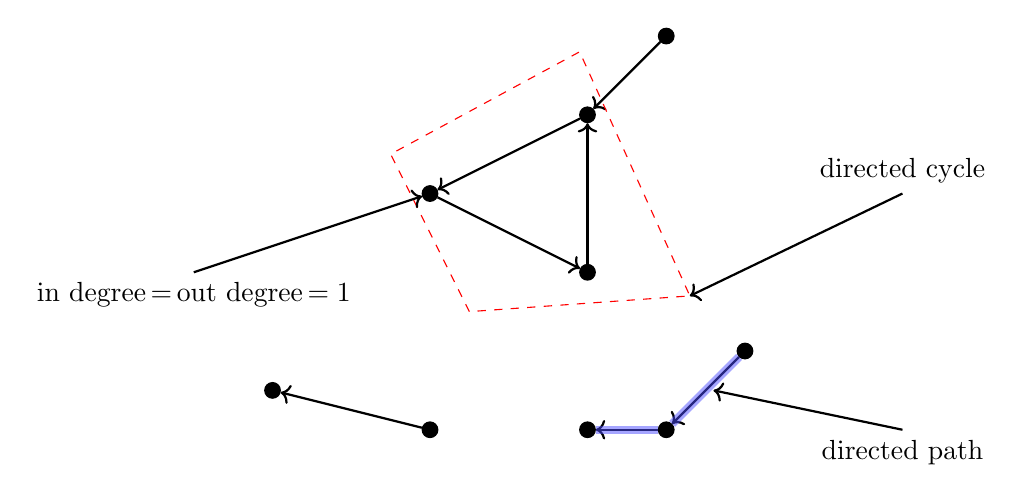
\begin{tikzpicture}[node distance=2cm, every edge/.style={draw=black,very thick}]
    % nodes
    \node[circle,draw,fill=black,inner sep=2pt] (v1) at(0,0) {};
    \node[circle,draw,fill=black,inner sep=2pt] (v2) at(0,3) {};
    \node[circle,draw,fill=black,inner sep=2pt] (v3) at(2,2) {};
    \node[circle,draw,fill=black,inner sep=2pt] (v4) at(3,0) {};
    \node[circle,draw,fill=black,inner sep=2pt] (v5) at(2,4) {};
    \node[circle,draw,fill=black,inner sep=2pt] (v6) at(3,5) {};
    \node[circle,draw,fill=black,inner sep=2pt] (v7) at(4,1) {};
    \node[circle,draw,fill=black,inner sep=2pt] (v9) at(2,0) {};
    \node[circle,draw,fill=black,inner sep=2pt] (v8) at(-2,0.5) {};
    % degree
    \draw[thick,->] (v1) -- (v8);
    \draw[thick,->] (v2) -- (v3);
    \draw[thick,->] (v3) -- (v5);
    \draw[thick,->] (v6) -- (v5);
    \draw[thick,<-] (v2) -- (v5);
    \draw[thick,->] (v7) -- (v4);
    \draw[thick,->] (v4) -- (v9);
    \draw[line width=3pt, blue!70!white, opacity=0.5] (v7) -- (v4);
    \draw[line width=3pt, blue!70!white, opacity=0.5] (v4) -- (v9);


    \draw[dashed,red] (0.5,1.5) -- (-0.5,3.5) -- (1.9,4.8) -- (3.3,1.7) -- (0.5,1.5);

    \draw[->,thick] (-3,2)node[below]{in degree$\,=\,$out degree$\,=1$} -- (v2);
    \draw[->,thick] (6,3)node[above]{directed cycle} -- (3.3,1.7);
    \draw[->,thick] (6,0)node[below]{directed path} -- (3.6,0.5);
    \end{tikzpicture}
\end{center}

\begin{lstlisting}
class Digraph:
    def __init__(self, num_vertices: int):
        self.num_vertices = num_vertices
        self.adj = [[] for v in range(num_vertices)]

    def add_edge(self, vertex1: int, vertex2: int) -> None:
        self.adj[vertex1].append(vertex2)

    def get_adj_list(self, vertex: int) -> list:
        return self.adj[vertex].copy()

    def get_num_vertices(self) -> int:
        return self.num_vertices
\end{lstlisting}

\subsubsection*{DFS and BFS}
\begin{lstlisting}
from Digraph import Digraph

class DirectedDFS:
    def __init__(self, graph: Digraph, start_vertex: int) -> None:
        self.visited = [False] * graph.get_num_vertices()
        self.edge_to = [-1] * graph.get_num_vertices()
        self.start_vertex = start_vertex
        self.dfs(graph, start_vertex)

    def dfs(self, graph: Digraph, vertex: int) -> None:
        self.visited[vertex] = True
        for neighbor in graph.get_adj_list(vertex):
            if not self.visited[neighbor]:
                self.edge_to[neighbor] = vertex
                self.dfs(graph, neighbor)
\end{lstlisting}

\begin{lstlisting}
from Digraph import Digraph
from Queue import Queue

class DirectedBFS:
    def __init__(self, graph: Digraph, start_vertex: int) -> None:
        self.dist_to_source = [-1] * graph.get_num_vertices()
        self.edge_to = [-1] * graph.get_num_vertices()
        self.start_vertex = start_vertex
        self.bfs(graph, start_vertex)

    def bfs(self, graph: Digraph, vertex: int) -> None:
        queue = Queue()
        queue.enqueue(vertex)
        self.dist_to_source[vertex] = 0
        while not queue.is_empty():
            vertex = queue.dequeue()
            for neighbor in graph.get_adj_list(vertex):
                if self.dist_to_source[neighbor] == -1:
                    queue.enqueue(neighbor)
                    self.dist_to_source[neighbor] = self.dist_to_source[vertex] + 1
                    self.edge_to[neighbor] = vertex
\end{lstlisting}

\subsubsection*{Topological Order}
Precedence scheduling: Given a set of tasks to be completed with precedence constraints, in which order should we schedule the tasks?\\
How:
\begin{itemize}
    \item Check the graph is a DAG
    \item Run depth-first search
    \item Return vertices in reverse post-order
\end{itemize}
Challenge: Given a directed acyclic graph (DAG), redraw it so that all edges point upwards.

\begin{center}
    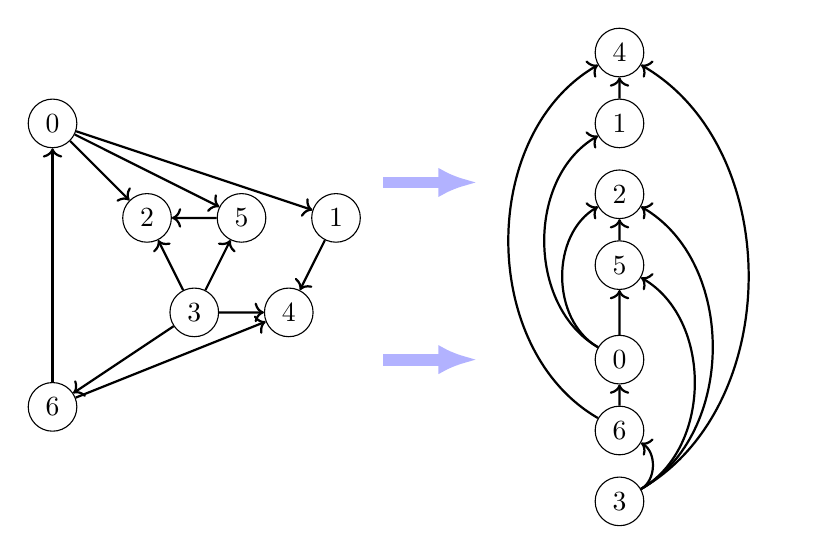
\begin{tikzpicture}[=>=latex, scale = 0.6]
        \node[circle, draw, black] (0) at (0,0){0};
        \node[circle, draw, black] (1) at (6,-2){1};
        \node[circle, draw, black] (2) at (2,-2){2};
        \node[circle, draw, black] (3) at (3,-4){3};
        \node[circle, draw, black] (4) at (5,-4){4};
        \node[circle, draw, black] (5) at (4,-2){5};
        \node[circle, draw, black] (6) at (0,-6){6};
        %array
        \draw[thick,->] (0) -- (1);
        \draw[thick,->] (0) -- (2);
        \draw[thick,->] (0) -- (5);
        \draw[thick,->] (1) -- (4);
        \draw[thick,->] (3) -- (2);
        \draw[thick,->] (3) -- (4);
        \draw[thick,->] (3) -- (5);
        \draw[thick,->] (3) -- (6);
        \draw[thick,->] (5) -- (2);
        \draw[thick,->] (6) -- (0);
        \draw[thick,->] (6) -- (4);
        %mid array
        \draw[-{Latex[length=0.5cm]},line width=0.15cm,blue!30](7,-1.25)to(9,-1.25);
        \draw[-{Latex[length=0.5cm]},line width=0.15cm,blue!30](7,-5)to(9,-5);
        %right part
        \node[circle, draw, black] (0) at (12,-5){0};
        \node[circle, draw, black] (1) at (12,0){1};
        \node[circle, draw, black] (2) at (12,-1.5){2};
        \node[circle, draw, black] (3) at (12,-8){3};
        \node[circle, draw, black] (4) at (12,1.5){4};
        \node[circle, draw, black] (5) at (12,-3){5};
        \node[circle, draw, black] (6) at (12,-6.5){6};
        %array
        \draw[thick, ->, bend left = 60] (0) to (1);
        \draw[thick, ->, bend left = 60] (0) to (2);
        \draw[thick, ->] (0) -- (5);
        \draw[thick, ->] (1) -- (4);
        \draw[thick, ->, bend right = 60] (3) to (2);
        \draw[thick, ->, bend right = 60] (3) to (4);
        \draw[thick, ->, bend right = 60] (3) to (5);
        \draw[thick, ->, bend right = 60] (3) to (6);
        \draw[thick, ->] (5) -- (2);
        \draw[thick, ->] (6) -- (0);
        \draw[thick, ->, bend left = 60] (6) to (4);
    \end{tikzpicture}
\end{center}

\begin{lstlisting}
from Digraph import Digraph
from Stack import Stack

class TopologicalSort:
    def __init__(self, graph: Digraph):
        self.visited = [False] * graph.get_num_vertices()
        self.reverse_post = Stack()
        for vertex in range(graph.get_num_vertices()):
            if not self.visited[vertex]:
                self.dfs(graph, vertex)

    def dfs(self, graph: Digraph, vertex: int):
        self.visited[vertex] = True
        for neighbor in graph.get_adj_list(vertex):
            if not self.visited[neighbor]:
                self.dfs(graph, neighbor)
        self.reverse_post.push(vertex)

    def get_topological_order(self) -> list:
        topo_order = []
        while not self.reverse_post.is_empty():
            topo_order.append(self.reverse_post.pop())
        return topo_order
\end{lstlisting}

\subsubsection*{Directed Cycle Detection}
Challenge: Is a given digraph $G$ a DAG?\\
How: 
\begin{itemize}
    \item Visit $G$ using DFS
    \item Keep track of vertices whose recursive \verb|dfs()| call has not completed yet
    \item If a call is made to a vertex with an open \verb|dfs()| call, $G$ is not a DAG
\end{itemize}

\begin{lstlisting}
from Digraph import Digraph

class DirectedCycle:
    def __init__(self, graph: Digraph) -> None:
        self.visited = [False] * graph.get_num_vertices()
        self.on_call_stack = [False] * graph.get_num_vertices()
        self.cycle_detected = False
        for vertex in range(graph.get_num_vertices()):
            if not self.visited[vertex]:
                self.dfs(graph, vertex)

    def dfs(self, graph: Digraph, vertex: int) -> None:
        self.visited[vertex] = True
        self.on_call_stack[vertex] = True
        for neighbor in graph.get_adj_list(vertex):
            if not self.visited[neighbor]:
                self.dfs(graph, neighbor)
            elif self.on_call_stack[neighbor]:
                self.cycle_detected = True
                return
            self.on_call_stack[vertex] = False

    def has_cycle(self) -> bool:
        return self.cycle_detected
\end{lstlisting}

\subsubsection*{Strongly-Connected Component}
Definition: Vertices $v$ and $w$ are strongly connected if there is both a directed path from $v$ to $w$ and a directed path from $w$ to $v$\\
Definition: A strong component is a maximal subset of strongly-connected vertices. Strong connectivity is an equivalence relation\\
\subsubsection*{Kosaraju-Sharir Algorithm}
Reverse graph: Strong components in $G$ are same as in $G^R$.\\
Two phase approach:
\begin{itemize}
    \item Compute topological order (i.e., reverse post-order) in $G^R$
    \item Run DFS in $G$, visiting unmarked vertices in reverse post-order of $G^R$
\end{itemize}

\begin{lstlisting}
class Digraph:
    def __init__(self, num_vertices: int):
        self.num_vertices = num_vertices
        self.adj = [[] for _ in range(num_vertices)]

    def add_edge(self, vertex1: int, vertex2: int) -> None:
        self.adj[vertex1].append(vertex2)

    def get_adj_list(self, vertex: int) -> list:
        return self.adj[vertex].copy()

    def get_num_vertices(self) -> int:
        return self.num_vertices

    def reverse(self) -> 'Digraph':
        new_adj = [[] for _ in range(self.num_vertices)]
        for vertex in range(self.num_vertices):
            for neighbor in self.get_adj_list(vertex):
                new_adj[neighbor].append(vertex)
        return Digraph(self.num_vertices)._from_adj_lists(new_adj)

    def _from_adj_lists(self, adj: list) -> 'Digraph':
        self.adj = adj
        return self
\end{lstlisting}

\begin{lstlisting}
from Digraph import Digraph
from TopologicalSort import TopologicalSort

class StronglyConnectedComponents:
    def __init__(self, graph: Digraph):
        self.visited = [False] * graph.get_num_vertices()
        self.scc = [-1] * graph.get_num_vertices()
        self.count = 0
        dfs_order = TopologicalSort(graph.reverse()).get_topological_order()
        for vertex in dfs_order:
            if not self.visited[vertex]:
                self.dfs(graph, vertex)
                self.count += 1

    def dfs(self, graph: Digraph, vertex: int):
        self.visited[vertex] = True
        self.scc[vertex] = self.count
        for neighbor in graph.get_adj_list(vertex):
            if not self.visited[neighbor]:
                self.dfs(graph, neighbor)

    def same_scc(self, vertex1: int, vertex2: int) -> bool:
        return self.scc[vertex1] == self.scc[vertex2]
\end{lstlisting}

\subsection{Minimum Spanning Tree}
\subsubsection*{Greedy Algorithm}
A cut in a graph is a partition of its vertices into two (nonempty) sets.\\
A crossing edge connects a vertex in one set with a vertex in the other.\\
Property: given any cut, the crossing edge of min weight is in the MST\\
Key idea:
\begin{itemize}
    \item Start with all edges colored grey
    \item Find a cut with no black-crossing edges
    \item Color its min-weight edge black
    \item Repeat until $V-1$ edges are colored black
\end{itemize}

\begin{lstlisting}
class Edge:
    def __init__(self, vertex1: int, vertex2: int, weight: float) -> None:
        self.vertex1 = vertex1
        self.vertex2 = vertex2
        self.weight = weight

    def get_vertex1(self) -> int:
        return self.vertex1

    def get_vertex2(self) -> int:
        return self.vertex2

    def get_other_vertex(self, vertex: int) -> int:
        if vertex == self.vertex1:
            return self.vertex2
        if vertex == self.vertex2:
            return self.vertex1

    def __lt__(self, other: 'Edge') -> bool:
        return self.weight < other.weight

    def __gt__(self, other: 'Edge') -> bool:
        return self.weight > other.weight

    def __eq__(self, other: 'Edge') -> bool:
        return self.weight == other.weight
    
    def __le__(self, other: 'Edge') -> bool:
        return self.weight <= other.weight
    
    def __ge__(self, other: 'Edge') -> bool:
        return self.weight >= other.weight
\end{lstlisting}

\begin{lstlisting}
from Edge import Edge

class EdgeWeightedGraph:
    def __init__(self, num_vertices: int) -> None:
        self.num_vertices = num_vertices
        self.adj = [[] for _ in range(num_vertices)]

    def add_edge(self, edge: Edge) -> None:
        vertex1 = edge.get_vertex1()
        vertex2 = edge.get_vertex2()
        self.adj[vertex1].append(edge)
        self.adj[vertex2].append(edge)

    def get_num_vertices(self) -> int:
        return self.num_vertices

    def get_adj_list(self, vertex: int) -> list:
        return self.adj[vertex]
\end{lstlisting}

\subsubsection*{Kruskal's algorithm}
Key idea:
\begin{itemize}
    \item Consider edges in ascending order of weight
    \item Add the next edge to the MST, unless doing so would create a cycle
    \item Stop when all the edges have been considered (or when $V-1$ edges have been added)
\end{itemize}

\begin{lstlisting}
class MinPriorityQueue:
    def __init__(self) -> None:
        self.heap = [None]
        self.tail = 0

    def enqueue(self, key) -> None:
        self.heap.append(key)
        self.tail += 1
        self._swim(self.tail)

    def dequeue(self):
        if self.tail == 0:
            return None
        min = self.heap[1]
        self.heap[1], self.heap[self.tail] = self.heap[self.tail], self.heap[1]
        self.heap[self.tail] = None
        self.tail -= 1
        self._sink(1)
        self.heap.pop()
        return min

    def _swim(self, i: int) -> None:
        while i > 1 and self.heap[i//2] > self.heap[i]:
            self.heap[i], self.heap[i//2] = self.heap[i//2], self.heap[i]
            i //= 2

    def _sink(self, i: int) -> None:
        while 2*i <= self.tail:
            j = 2*i
            if j < self.tail and self.heap[j] > self.heap[j+1]:
                j += 1
            if self.heap[i] <= self.heap[j]:
                break
            self.heap[i], self.heap[j] = self.heap[j], self.heap[i]
            i = j

    def is_empty(self) -> bool:
        return len(self.heap) == 1
\end{lstlisting}

\begin{lstlisting}
from Edge import Edge

class UnionFind:
\end{lstlisting}

\begin{lstlisting}
from EdgeWeightedGraph import EdgeWeightedGraph
from Queue import Queue
from MinPriorityQueue import MinPriorityQueue
from UnionFind import UnionFind
from Edge import Edge

class KruskalMST:
    def __init__(self, graph: EdgeWeightedGraph) -> None:
        self.mst = Queue()
        self.pq = MinPriorityQueue()
        for edge in graph.get_adj_list():
            self.pq.enqueue(edge)

        uf = UnionFind(graph.get_num_vertices())
        while not self.pq.is_empty() and self.mst.size() < graph.num_vertices-1:
            edge = self.pq.dequeue()
            vertex1 = edge.get_vertex1()
            vertex2 = edge.get_vertex2()
            if not uf.connected():
                uf.union(vertex1, vertex2)
                self.mst.enqueue(edge)

    def edges(self):
        return self.mst
\end{lstlisting}
\begin{spacing}{1.5}
\begin{tabularx}{1\textwidth}{|X|X|X|X|X|}
    \hline
    \textbf{\color{blue}Worst Case}&\textbf{Build the priority queue} & \textbf{Delete min} & \textbf{Union} & \textbf{Find (connected)}\\
    \hline
    \textbf{Frequency}&$1$&$E$&$V$&$E$\\
    \hline
    \textbf{Cost per operation}&$E\,\log\,E$&$\log\,E$&$\log\,V$&$\log\,V$\\
    \hline
\end{tabularx}
\end{spacing}

\subsubsection*{Prim's Algorithm}
Key idea:
\begin{itemize}
    \item Start with vertex $0$ and greedily grow tree $T$
    \item Add to $T$ the min-weighted edge with exactly one endpoint in $T$
    \item Stop when $V-1$ edges have been added
\end{itemize}

\begin{lstlisting}
from EdgeWeightedGraph import EdgeWeightedGraph
from Queue import Queue
from MinPriorityQueue import MinPriorityQueue
from Edge import Edge

class LazyPrimMST:
    def __init__(self, graph: EdgeWeightedGraph) -> None:
        self.visited = [False] * graph.get_num_vertices()
        self.mst = Queue()
        self.pq = MinPriorityQueue()
        self.visit(graph, 0)

        while not self.pq.is_empty() and self.mst.size() < graph.get_num_vertices() - 1:
            edge = self.pq.dequeue()
            vertex1 = edge.get_vertex1()
            vertex2 = edge.get_vertex2()
            if self.visited[vertex1] and self.visited[vertex2]:
                continue
            self.mst.enqueue(edge)
            if not self.visited[vertex1]:
                self.visit(graph, vertex1)
            if not self.visited[vertex2]:
                self.visit(graph, vertex2)

    def visit(self, graph: EdgeWeightedGraph, vertex: int):
        self.visited[vertex] = True
        for edge in graph.get_adj_list(vertex):
            if not self.visited[edge.get_other_vertex(vertex)]:
                self.pq.enqueue(edge)

    def get_mst_edges(self) -> Queue:
        return self.mst
\end{lstlisting}

\begin{spacing}{1.5}
\begin{tabularx}{1\textwidth}{|X|X|X|}
    \hline
    \textbf{\color{blue}Worst Case}&\textbf{Delete min} & \textbf{Insert}\\
    \hline
    \textbf{Frequency}&$E$&$E$\\
    \hline
    \textbf{Cost per operation}&$\log\,E$&$\log\,E$\\
    \hline
\end{tabularx}
\end{spacing}

\subsection{Shortest Path}
\subsubsection*{Problem Formulation}

Shortest path from one vertex $s$ to any other in $G$
\begin{itemize}
    \item Simplifying assumption: shortest paths from $s$ to each vertex $v$ in $G$ exist
\end{itemize}

Generic algorithm to compute SPT from $s$:
\begin{enumerate}
    \item Initialise \verb|distTo[s]=0|
    \item Initialise \verb|distTo[v]=|$\infty$ for all other vertices
    \item Repeat \verb|relax(e)| for any edge $e:v\to w$, until there are no more edges $e$ for which \verb|distTo[v]| \verb|+ e.weight()| \verb| < distTo[w]|
\end{enumerate}

\begin{lstlisting}
class WeightedEdge:
    def __init__(self, start_vertex: int, end_vertex: int, weight: float) -> None:
        self.start_vertex = start_vertex
        self.end_vertex = end_vertex
        self.weight = weight

    def get_start_vertex(self) -> int:
        return self.start_vertex

    def get_end_vertex(self) -> int:
        return self.end_vertex

    def get_weight(self) -> float:
        return self.weight

    def __lt__(self, other: 'WeightedEdge') -> bool:
        return self.weight < other.weight

    def __gt__(self, other: 'WeightedEdge') -> bool:
        return self.weight > other.weight

    def __eq__(self, other: 'WeightedEdge') -> bool:
        return self.weight == other.weight

    def __le__(self, other: 'WeightedEdge') -> bool:
        return self.weight <= other.weight

    def __ge__(self, other: 'WeightedEdge') -> bool:
        return self.weight >= other.weight
\end{lstlisting}

\begin{lstlisting}
from WeightedEdge import WeightedEdge

class EdgeWeightedDigraph:
    def __init__(self, num_vertices: int) -> None:
        self.num_vertices = num_vertices
        self.adj = [[] for _ in range(num_vertices)]

    def add_edge(self, edge: WeightedEdge) -> None:
        vertex = edge.get_start_vertex()
        self.adj[vertex].append(edge)

    def get_num_vertices(self) -> int:
        return self.num_vertices

    def get_adj_list(self, vertex: int) -> list:
        return self.adj[vertex]
\end{lstlisting}


\subsubsection*{Dijkstra's Algorithm}
Assumption: Digraph has non-negative weights\\
Key idea:
\begin{itemize}
    \item Consider vertices in increasing order of distance from $s$
    \item Add vertex to the SPT and relax all its outgoing edges
\end{itemize}

\begin{lstlisting}
    class MinPriorityQueue:
    def __init__(self) -> None:
        self.key = [None]
        self.value = [None]
        self.tail = 0

    def enqueue(self, key, value) -> None:
        self.key.append(key)
        self.value.append(value)
        self.tail += 1
        self._swim(self.tail)

    def dequeue(self) -> object:
        if self.tail == 0:
            return None
        minimum = self.value[1]
        self.key[1], self.key[self.tail] = self.key[self.tail], self.key[1]
        self.value[1], self.value[self.tail] = self.value[self.tail], self.value[1]
        self.key[self.tail] = None
        self.value[self.tail] = None
        self.tail -= 1
        self._sink(1)
        self.key.pop()
        self.value.pop()
        return minimum

    def _swim(self, i: int) -> None:
        while i > 1 and self.key[i//2] > self.key[i]:
            self.key[i], self.key[i//2] = self.key[i//2], self.key[i]
            self.value[i], self.value[i//2] = self.value[i//2], self.value[i]
            i //= 2

    def _sink(self, i: int) -> None:
        while 2*i <= self.tail:
            j = 2*i
            if j < self.tail and self.key[j] > self.key[j+1]:
                j += 1
            if self.key[i] <= self.key[j]:
                break
            self.key[i], self.key[j] = self.key[j], self.key[i]
            self.value[i], self.value[j] = self.value[j], self.value[i]
            i = j

    def is_empty(self) -> bool:
        return len(self.key) == 1

    def contains(self, value: int) -> bool:
        return value in self.value

    def decrease_key(self, key, value: int) -> None:
        for i in range(len(self.value)):
            if self.value[i] == value:
                self.key[i] = key
                self._swim(i)
                break
\end{lstlisting}

\begin{lstlisting}
from EdgeWeightedDigraph import EdgeWeightedDigraph
from WeightedEdge import WeightedEdge
from Stack import Stack
from MinPriorityQueue import MinPriorityQueue
import math

class DijkstraSP:
    def __init__(self, graph: EdgeWeightedDigraph, start_vertex: int) -> None:
        self.dist_to = [math.inf] * graph.get_num_vertices()
        self.edge_to = [None] * graph.get_num_vertices()
        self.dist_to[start_vertex] = 0

        self.pq = MinPriorityQueue()
        self.pq.enqueue(0, start_vertex)

        while not self.pq.is_empty():
            vertex = self.pq.dequeue()
            for edge in graph.get_adj_list(vertex):
                self.relax(edge)

    def get_dist_to(self, vertex: int) -> float:
        return self.dist_to[vertex]

    def get_path_to(self, vertex) -> list:
        path = Stack()
        edge = self.edge_to[vertex]
        while edge is not None:
            path.push(edge)
            edge = self.edge_to[edge.get_start_vertex()]
        return path

    def relax(self, edge: WeightedEdge):
        start_vertex = edge.get_start_vertex()
        end_vertex = edge.get_end_vertex()
        if self.dist_to[start_vertex] + edge.get_weight() < self.dist_to[end_vertex]:
            self.dist_to[end_vertex] = self.dist_to[start_vertex] + \
                edge.get_weight()
            self.edge_to[end_vertex] = edge
            if self.pq.contains(end_vertex):
                self.pq.decrease_key(self.dist_to[end_vertex], end_vertex)
            else:
                self.pq.enqueue(self.dist_to[end_vertex], end_vertex)
\end{lstlisting}

\begin{spacing}{1.5}
\begin{tabularx}{1\textwidth}{|X|X|X|X|X|}
    \hline
    \textbf{\color{blue}PQ implementation}&\textbf{insert()} & \textbf{delMin()}& \textbf{decreaseKey()}&\textbf{total} \\
    \hline
    \textbf{Binary heap}&$\log\,V$&$\log\,V$&$\log\,V$&$E\log\,V$\\
    \hline
\end{tabularx}
\end{spacing}

\subsubsection*{Edge-Weighted DAG Algorithm}
Assumption: Digraph is acyclic (DAG)\\
Key idea:
\begin{itemize}
    \item Consider vertices in topological order
    \item Add vertex to the SPT and relax all its outgoing edges
\end{itemize}

\begin{lstlisting}
from WeightedEdge import WeightedEdge
from EdgeWeightedDigraph import EdgeWeightedDigraph
from Stack import Stack

class TopologicalSort:
    def __init__(self, graph: EdgeWeightedDigraph):
        self.visited = [False] * graph.get_num_vertices()
        self.reverse_post = Stack()
        for vertex in range(graph.get_num_vertices()):
            if not self.visited[vertex]:
                self.dfs(graph, vertex)

    def dfs(self, graph: EdgeWeightedDigraph, vertex: int):
        self.visited[vertex] = True
        for edge in graph.get_adj_list(vertex):
            if not self.visited[edge.get_end_vertex()]:
                self.dfs(graph, edge.get_end_vertex())
        self.reverse_post.push(vertex)

    def get_topological_order(self) -> list:
        topo_order = []
        while not self.reverse_post.is_empty():
            topo_order.append(self.reverse_post.pop())
        return topo_order
\end{lstlisting}

\begin{lstlisting}
from EdgeWeightedDigraph import EdgeWeightedDigraph
from WeightedEdge import WeightedEdge
from TopologicalSort import TopologicalSort
from Stack import Stack
import math

class AcyclicSP:
    def __init__(self, graph: EdgeWeightedDigraph, start_vertex: int) -> None:
        self.dist_to = [math.inf] * graph.get_num_vertices()
        self.edge_to = [None] * graph.get_num_vertices()
        self.dist_to[start_vertex] = 0

        topological_order = TopologicalSort(graph).get_topological_order()

        while len(topological_order) > 0:
            vertex = topological_order.pop(0)
            for edge in graph.get_adj_list(vertex):
                self.relax(edge)

    def get_dist_to(self, vertex: int) -> float:
        return self.dist_to[vertex]

    def get_path_to(self, vertex) -> list:
        path = Stack()
        edge = self.edge_to[vertex]
        while edge is not None:
            path.push(edge)
            edge = self.edge_to[edge.get_start_vertex()]
        return path

    def relax(self, edge: WeightedEdge):
        start_vertex = edge.get_start_vertex()
        end_vertex = edge.get_end_vertex()
        if self.dist_to[start_vertex] + edge.get_weight() < self.dist_to[end_vertex]:
            self.dist_to[end_vertex] = self.dist_to[start_vertex] + \
                edge.get_weight()
            self.edge_to[end_vertex] = edge
\end{lstlisting}

\textbf{Cost: Dominated by computation of topological sort on DAG $(E+V)$}

\subsubsection*{Bellman-Ford Algorithm}
Assumption: Digraph has non-negative cycles\\
Key idea 
\begin{itemize}
    \item Repeat V times: relax all edges
\end{itemize}

\begin{lstlisting}
from EdgeWeightedDigraph import EdgeWeightedDigraph
from WeightedEdge import WeightedEdge
from Stack import Stack
import math

class BellmanFordSP:
    def __init__(self, graph: EdgeWeightedDigraph, start_vertex: int) -> None:
        self.dist_to = [math.inf] * graph.get_num_vertices()
        self.edge_to = [None] * graph.get_num_vertices()
        self.dist_to[start_vertex] = 0

        for _ in range(graph.get_num_vertices()):
            for vertex in range(graph.get_num_vertices()):
                for edge in graph.get_adj_list(vertex):
                    self.relax(edge)

    def get_dist_to(self, vertex: int) -> float:
        return self.dist_to[vertex]

    def get_path_to(self, vertex) -> list:
        path = Stack()
        edge = self.edge_to[vertex]
        while edge is not None:
            path.push(edge)
            edge = self.edge_to[edge.get_start_vertex()]
        return path

    def relax(self, edge: WeightedEdge):
        start_vertex = edge.get_start_vertex()
        end_vertex = edge.get_end_vertex()
        if self.dist_to[start_vertex] + edge.get_weight() < self.dist_to[end_vertex]:
            self.dist_to[end_vertex] = self.dist_to[start_vertex] + \
                edge.get_weight()
            self.edge_to[end_vertex] = edge
\end{lstlisting}
Practical improvement:
\begin{itemize}
    \item If \verb|distTo[v]| does not change during pass $i$, no need to relax any outgoing edge from $v$ in pass $i+1$
    \item Maintain a queue of vertices whose \verb|distTo[]| changed
\end{itemize}

\textbf{Cost: Proportional to $E\times V$, but only in worst case}

\subsubsection*{Single-Source Shortest Path Summary}
\begin{spacing}{1.5}
\begin{tabularx}{1\textwidth}{|X|X|X|X|X|}
    \hline
    \textbf{Algorithm}&\textbf{Restriction} & \textbf{Typical case}& \textbf{Worst case}&\textbf{Extra space} \\
    \hline
    Dijkstra (binary heap)&No negative weights&$E\,\log\,V$&$E\,\log\,V$&$V$\\
    \hline
    Edge-weighted DAG (topological sort)&No cycles&$E+V$&$E+V$&$V$\\
    \hline
    Bellman-Ford&No negative cycles&$EV$&$EV$&$V$\\
    \hline
    Bellman-Ford (queue based)&No negative cycles&$E+V$&$EV$&$V$\\
    \hline
\end{tabularx}
\end{spacing}

\section{String Algorithms}
String: Sequence of characters.\\
Character: Digit from a fixed alphabet of size $R$ (radix).\\
String operations:
\begin{itemize}
    \item Length: Number of characters.
    \item Indexing: Get the $i$th character.
    \item Substring extraction: Get a contiguous subsequence of characters.
    \item String concatenation: Append a string to the end of another string.
\end{itemize}

\subsection{String Sorting Algorithms}
\subsubsection*{Key-Index Counting}
Assumption: Keys are integers in $[0, R-1]$. (One character long)\\
Goal: Sort an array \verb|a[]| of $N$ integers with values in $[0, R-1]$.\\
Steps:
\begin{enumerate}
    \item Count frequencies of each value in $R$ using key as index
    \item Compute frequency cumulates (to specify destinations)
    \item Access cumulates using key as index and move items
    \item Copy back into original array
\end{enumerate}

\begin{lstlisting}
def key_indexed_counting(char_list: list, radix: int):
    N = len(char_list)
    count = [0] * (radix + 1)
    aux = [''] * N

    for i in range(N):
        count[ord(char_list[i]) + 1] += 1

    for r in range(radix):
        count[r + 1] += count[r]

    for i in range(N):
        aux[count[ord(char_list[i])]] = char_list[i]
        count[ord(char_list[i])] += 1

    for i in range(N):
        char_list[i] = aux[i]
\end{lstlisting}

\begin{spacing}{1.5}
\begin{tabularx}{1\textwidth}{|X|X|X|X|X|}
    \hline
    &\textbf{In place} & \textbf{Stable} & \textbf{Time} & \textbf{Space}\\
    \hline
    \textbf{Key-Index Counting}&&\centering\checkmark&$\sim N+R$&$\sim N+R$\\
    \hline
\end{tabularx}
\end{spacing}


\subsubsection*{LSD Radix Sort}
Least-significant-digit first string (radix) sort. (means from right to left)\\
\newline
Assumption: Keys all have the same (small) length $D$
Basic Idea
\begin{itemize}
    \item Consider each character in turn, from right to left
    \item At each pass, use key-indexed counting on $d$th character to sort (stably)
\end{itemize}

\begin{lstlisting}
def LSDsort(str_list: list, radix: int):
    N = len(str_list)
    W = len(str_list[0])

    for d in range(W-1, -1, -1):
        count = [0] * (radix + 1)
        aux = [''] * N

        for i in range(N):
            count[ord(str_list[i][d]) + 1] += 1

        for r in range(radix):
            count[r + 1] += count[r]

        for i in range(N):
            aux[count[ord(str_list[i][d])]] = str_list[i]
            count[ord(str_list[i][d])] += 1

        for i in range(N):
            str_list[i] = aux[i]
\end{lstlisting}

\begin{spacing}{1.5}
\begin{tabularx}{1\textwidth}{|X|X|X|X|X|}
    \hline
    &\textbf{In place} & \textbf{Stable} & \textbf{Time} & \textbf{Space}\\
    \hline
    \textbf{LSD Radix Sort}&&\centering\checkmark&$\sim W\times (N+R)$&$\sim (N+R)$\\
    \hline
\end{tabularx}
\end{spacing}

\subsubsection*{MSD Radix Sort}
Most-significant-digit first string (radix) sort (left to right)\\
\newline
Basic Idea:
\begin{itemize}
    \item Partition input into R pieces according to first character (use key-indexed counting to sort)
    \item Recursively sort all strings that start with the same character
\end{itemize}

\begin{lstlisting}
def MSDsort(str_list: list, aux, lo: int, hi: int, d: int, radix: int):
    if hi <= lo:
        return
    count = [0] * (radix + 2)

    for i in range(lo, hi):
        count[ord(str_list[i][d]) + 2] += 1

    for r in range(radix+1):
        count[r+1] += count[r]

    for i in range(lo, hi):
        aux[count[ord(str_list[i][d]) + 1]] = str_list[i]
        count[ord(str_list[i][d]) + 1] += 1

    for i in range(lo, hi):
        str_list[i] = aux[i - lo]

    for r in range(radix):
        MSDsort(str_list, aux, lo + count[r], lo + count[r+1] - 1, d+1, radix)
\end{lstlisting}

\begin{spacing}{1.5}
\begin{tabularx}{1\textwidth}{|X|X|X|X|X|X|}
    \hline
    &\textbf{In place} & \textbf{Stable} & \textbf{Worst case time} & \textbf{Average case time} & \textbf{Space}\\
    \hline
    \textbf{LSD Radix Sort}&&\centering\checkmark&$\sim W\times N$&$\sim N\,\log_{R}N$&$\sim N+D\times R$\\
    \hline
\end{tabularx}
\end{spacing}

\subsection{String Search}
\subsubsection*{R-way Tries}
Key idea: tree representation of symbol table
\begin{itemize}
    \item Each node represents (i.e., stores) one character, not full keys
    \item Each node has exactly $R$ children, one for each possible character
\end{itemize}

\begin{center}
    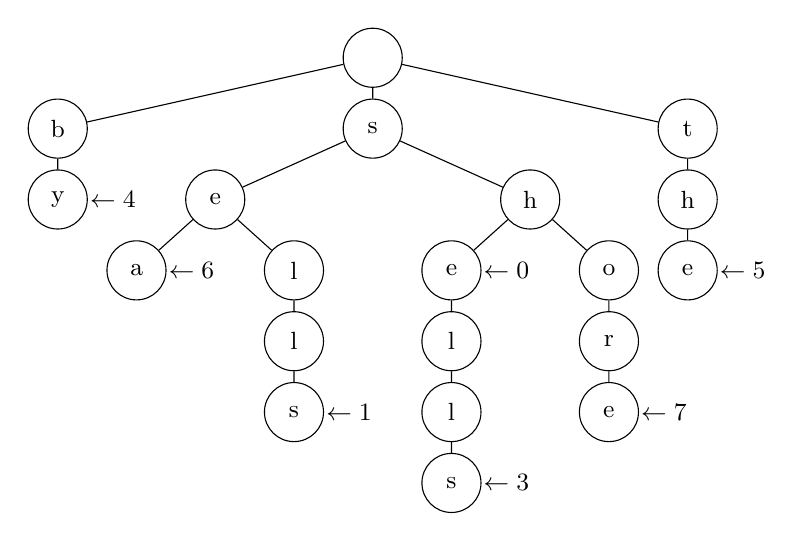
\begin{tikzpicture}[
        level 1/.style={sibling distance=4cm, level distance=0.9cm},
        level 2/.style={sibling distance=4cm, level distance=0.9cm},
        level 3/.style={sibling distance=2cm, level distance=0.9cm},
        every node/.style = {
        draw, circle, minimum size=0.75cm, font=\small
        }
        ]
        \node (root) {}
        child {
            node {b}
            child {
                node (by) {y}
            }
        }
        child {
            node {s}
            child {
                node {e}
                child {node (sea) {a}}
                child {
                    node {l}
                    child {
                        node {l}
                        child {
                            node (sells) {s}
                        }
                    }
                }
            }
            child {
                node {h}
                child {
                    node (she) {e}
                    child{
                        node {l}
                        child {
                            node {l}
                            child {
                                node (shells) {s}
                            }
                        }
                    }
                }
                child {
                    node {o}
                    child{
                        node {r}
                        child{
                            node (shore) {e}
                        }
                    }
                }
            }
        }
        child {
            node {t}
            child{
                node {h}
                child{
                    node (the) {e}
                }
            }
        };
    \node[right=0cm and -0.15cm of by, draw=none] {$\leftarrow 4$};
    \node[right=0cm and -0.15cm of sea, draw=none] {$\leftarrow 6$};
    \node[right=0cm and -0.15cm of sells, draw=none] {$\leftarrow 1$};
    \node[right=0cm and -0.15cm of shells, draw=none] {$\leftarrow 3$};
    \node[right=0cm and -0.15cm of she, draw=none] {$\leftarrow 0$};
    \node[right=0cm and -0.15cm of shore, draw=none] {$\leftarrow 7$};
    \node[right=0cm and -0.15cm of the, draw=none] {$\leftarrow 5$};
    \end{tikzpicture}
\end{center}

\begin{lstlisting}
class Node:
    def __init__(self, radix: int) -> None:
        self.value = None
        self.children = [None] * radix

    def set_children(self, i: int, node: 'Node') -> None:
        self.children[i] = node

    def get_children(self, i: int) -> 'Node':
        return self.children[i]

    def get_value(self) -> object:
        return self.value

    def set_value(self, value) -> None:
        self.value = value
\end{lstlisting}

\begin{lstlisting}
from Node import Node

class TrieST:
    def __init__(self, radix: int) -> None:
        self.radix = radix
        self.root = Node(radix)

    def put(self, key: str, value) -> None:
        self.root = self._put(self.root, key, value, 0)

    def _put(self, node: Node, key: str, value, d: int) -> Node:
        if node is None:
            node = Node(self.radix)
        if d == len(key):
            node.set_value(value)
            return node

        c = ord(key[d])
        node.set_children(c, self._put(node.get_children(c), key, value, d+1))
        return node

    def get(self, key: str) -> object:
        node = self._get(self.root, key, 0)
        if node is None:
            return None
        return node.get_value()

    def _get(self, node: Node, key: str, d: int) -> Node:
        if node is None:
            return None
        if d == len(key):
            return node

        c = ord(key[d])
        return self._get(node.get_children(c), key, d+1)
\end{lstlisting}

\begin{spacing}{1.5}
\begin{tabularx}{1\textwidth}{|X|X|X|}
    \hline
    \textbf{Search (hit)} & \textbf{Search (miss)} & \textbf{Space}\\
    \hline
    $L$&sub $L$&$N\times R$\\
    \hline
\end{tabularx}
\end{spacing}

\subsubsection*{3-way Tries}
Key idea
\begin{itemize}
    \item Each node represents (i.e., stores) one character, not full keys
    \item Each node has exactly 3 children: smaller (left), equal (middle), larger (right)
\end{itemize}

\begin{lstlisting}
class Node:
    def __init__(self):
        self.value = None
        self.char = ''
        self.left = None
        self.mid = None
        self.right = None
\end{lstlisting}

\begin{lstlisting}
from Node import Node

class TernarySearchTrieST:
    def __init__(self):
        self.root = Node()

    def put(self, key, value):
        self.root = self._put(self.root, key, value, 0)

    def _put(self, node, key, value, d):
        if not node:
            node = Node()
            node.char = key[d]

        c = key[d]
        if c < node.char:
            node.left = self._put(node.left, key, value, d)
        elif c > node.char:
            node.right = self._put(node.right, key, value, d)
        elif d < len(key) - 1:
            node.mid = self._put(node.mid, key, value, d + 1)
        else:
            node.value = value
        return node

    def get(self, key):
        node = self._get(self.root, key, 0)
        if node is None:
            return None
        return node.value

    def _get(self, node, key, d):
        if node is None:
            return None
        if d == len(key) - 1:
            return node

        c = key[d]
        if c < node.char:
            return self._get(node.left, key, d)
        elif c > node.char:
            return self._get(node.right, key, d)
        else:
            return self._get(node.mid, key, d + 1)
\end{lstlisting}

\begin{spacing}{1.5}
\begin{tabularx}{1\textwidth}{|X|X|}
    \hline
    \textbf{Time}  & \textbf{Space}\\
    \hline
    As fast as hashing, faster on search miss&$4N$\\
    \hline
\end{tabularx}
\end{spacing}

\subsubsection*{Extended API}
\verb|keys()|: iterate through all keys in sorted order\\
How to:
\begin{itemize}
    \item Do an in-order traversal of the trie
    \item Keep track of matched characters on the path from root to current node
    \item Add matched keys to a queue
\end{itemize}

\begin{lstlisting}
from Queue import Queue

class TrieST:
    def keys(self) -> Queue:
        queue = Queue()
        self.__collect(self.root, '', queue)
        return queue

    def __collect(self, node: Node, prefix: str, queue: Queue) -> None:
        if node is None:
            return
        if node.get_value() is not None:
            queue.enqueue(prefix)
        for c in range(self.radix):
            self.__collect(node.get_children(c), prefix + chr(c), queue)
\end{lstlisting}

\verb|keysWithPrefix(s)|: find all keys in the symbol table starting with \verb|s|\\
How to:
\begin{itemize}
    \item Do an in-order traversal of the trie, starting at the node $x$ matching \verb|s|
    \item Keep track of matched characters on the path from $x$ to current node
    \item Add matched keys to a queue
\end{itemize}

\begin{lstlisting}
class TrieST:
    def keys_with_prefix(self, s: str) -> Queue:
        queue = Queue()
        node = self._get(self.root, s, 0)
        self.__collect(node, s, queue)
        return queue
\end{lstlisting}

\verb|longestPrefixOf(s)|: find the longest key in the symbol table that is prefix of \verb|s|
How to:
\begin{itemize}
    \item Search for query string \verb|s|
    \item Keep track of longest key encountered
\end{itemize}

\begin{lstlisting}
class TrieST:
    def longest_prefix_of(self, prefix: str):
        length = self._search(self.root, prefix, 0, 0)
        return prefix[:length]

    def _search(self, node: Node, query: str, d: int, length: int):
        if node is None:
            return length
        if node.get_value() is not None:
            length = d
        if d == len(query):
            return length
        c = ord(query[d])
        return self._search(node.get_children(c), query, d+1, length)
\end{lstlisting}

\subsection{Substring Search}
Goal: Find a pattern of length $M$ in a text of length $N$ (usually $M<<N$).

\subsubsection*{Brute Force Algorithm}
Key idea: Use two indices $i$ and $j$ to scan the text and the pattern respectively. Compare the $j$th character in the pattern with the $(i+j)$th character in the text
\begin{itemize}
    \item In case of character match, move the index $j$ in the pattern of 1
    \item In case of character mismatch, move the search index $i$ in the text of 1 and restart the index $j$ in the pattern from the beginning
\end{itemize}

\begin{lstlisting}
def substring_search(pattern: str, text: str) -> int:
    pattern_len = len(pattern)
    text_len = len(text)

    for i in range(text_len - pattern_len + 1):
        j = 0
        while j < pattern_len:
            if text[i+j] != pattern[j]:
                break
            j += 1
        if j == pattern_len:
            return i
    return -1
\end{lstlisting}
\textbf{Cost (worst case)$\sim N\times M$}

\subsubsection*{Knuth-Morris-Pratt algorithm}
Key idea: Use a DFA as a string-searching machine.
\begin{itemize}
    \item Start in the initial state
    \item Read one character at a time from the input stream
    \item Consult the DFA transition table to know what state to go next (there is exactly one transition for each character in the alphabet)
    \item Pattern found if transition leads to final state
\end{itemize}
How to build the DFA from pattern
\begin{enumerate}
    \item Init. Create one state per character in the pattern, plus a final state
    \item Match transitions. If in state $j$ and next char \verb|c == pattern[j]|, go to state $j+1$
    \item Mismatch transitions.
    \begin{itemize}
        \item If in state j and next char \verb|c != pattern[j]|, then the last $j-1$ characters in input are \verb|pattern[1..j-1]|, followed by \verb|c|.
        \item To fill in \verb|DFA[c][j]|, simulate having \verb|pattern[1..j-1]| in input to the DFA, then take transition \verb|c|.
    \end{itemize}
\end{enumerate}

\begin{lstlisting}
class KnuthMorrisPrattSS:
    def __init__(self, pattern: str, radix: int) -> None:
        self.pattern_length = len(pattern)
        self.radix = radix
        self.DFA = [[0] * radix for _ in range(self.pattern_length)]
        self.build_DFA(pattern)

    def build_DFA(self, pattern: str) -> None:
        self.DFA[0][ord(pattern[0])] = 1
        X = 0
        for j in range(1, self.pattern_length):
            for c in range(self.radix):
                self.DFA[j][c] = self.DFA[X][c]
            self.DFA[j][ord(pattern[j])] = j+1
            X = self.DFA[X][ord(pattern[j])]

    def substring_search(self, text: str) -> int:
        text_length = len(text)
        i, j = 0, 0
        while i < text_length and j < self.pattern_length:
            j = self.DFA[j][ord(text[i])]
            i += 1
        if j == self.pattern_length:
            return i - self.pattern_length
        else:
            return -1
        
def substring_search(pattern: str, text: str) -> int:
    pattern_len = len(pattern)
    text_len = len(text)

    for i in range(text_len - pattern_len + 1):
        j = 0
        while j < pattern_len:
            if text[i+j] != pattern[j]:
                break
            j += 1
        if j == pattern_len:
            return i
    return -1
\end{lstlisting}

\begin{spacing}{1.5}
\begin{tabularx}{1\textwidth}{|X|X|}
    \hline
    \textbf{Construction of DFA} & \textbf{Substring search}\\
    \hline
    $\sim R\times M$&$\sim M+N$\\
    \hline
\end{tabularx}
\end{spacing}

\subsubsection*{Boyer-Moore Algorithm}
Key idea
\begin{itemize}
    \item Scan pattern from right to left
    \item Upon character mismatch, skip as many as $M$ text characters
\end{itemize}
How much to skip?
\begin{itemize}
    \item Case 1: mismatched character not present in pattern. Move $i$ beyond the mismatched position.
    \item Case 2: mismatched character in pattern. Precompute index of rightmost occurrence of mismatched character in pattern. Skip $i$ forward of (j - rightmost index)
\end{itemize}

\begin{lstlisting}
class BoyerMooreSS:
    def __init__(self, pattern: str, radix: int) -> None:
        self.pattern = pattern
        self.pattern_len = len(pattern)
        self.radix = radix
        self.index = [-1] * self.radix
        for i, c in enumerate(pattern):
            self.index[ord(c)] = i

    def substring_search(self, text: str) -> int:
        text_len = len(text)
        i = 0
        while i <= text_len - self.pattern_len:
            skip = 0
            j = self.pattern_len - 1
            while j >= 0:
                if self.pattern[j] != text[i + j]:
                    skip = max(1, j - self.index[ord(text[i + j])])
                    break
                else:
                    j -= 1

            i += skip
            if skip == 0:
                return i

        return -1
\end{lstlisting}

\begin{spacing}{1.5}
\begin{tabularx}{1\textwidth}{|X|X|X|}
    \hline
    \textbf{Pre-processing} & \textbf{Substring matching (Average)} & \textbf{Substring matching (Worst)}\\
    \hline
    $\sim M$&$\sim N/M$&$\sim M\times N$\\
    \hline
\end{tabularx}
\end{spacing}

\subsubsection*{Summary}
\begin{spacing}{1.5}
\begin{tabularx}{1\textwidth}{|X|X|X|}
    \hline
    \textbf{Brute force algorithm} & \textbf{Knuth-Morris-Pratt algorithm} & \textbf{Boyer-Moore algorithm}\\
    \hline
    $\sim N\times M$&$\sim N$&$\sim N/M$ (but worst case $N\times M$)\\
    \hline
\end{tabularx}
\end{spacing}

\subsection{Compression}
Lossless Compression\\
Goal:
\begin{itemize}
    \item Message. Given in input binary data (bit-stream) $B$.
    \item Compress. Generate a “compressed” representation $C(B)$.
    \item Expand. Reconstruct the original bitstream $B$ without loss.
\end{itemize}

\subsubsection*{Run-length Coding}
Key idea. Use counts to represent sequences of 0/1 bits\\
Representation. Use $n$-bit counts (e.g. $n=8$) to represent alternating runs of 0s and 1s.


\subsubsection*{Huffman Compression}
Key idea. Instead of encoding every character in alphabet using the same number of bits, use fewer bits for characters that appear more often, so to lower the total number of bits used.\\
\newline
Issue: ambiguity\\
Solution: Generate prefix-free code\\
\newline
How to: compression
\begin{itemize}
    \item Trie construction
    \item Trie transmission
    \item Compression based on leaves-to-root trie traversal
\end{itemize}
How to: prefix-free codes represented as binary trie
\begin{itemize}
    \item Chars in leaves
    \item Codeword is bit sequence path from root to leaf
\end{itemize}
How to: expansion
\begin{itemize}
    \item Start at the root of the trie and read one bit from the input stream at a time
    \item Go left if bit is 0, go right if 1
    \item Once on a leaf, emit corresponding key and restart the root
\end{itemize}

\end{document}